\documentclass[11pt]{article}

% macros.tex — GameTheory chapter notation
% Subset/extension of VegasCore macros.  Kept compatible so that, in a joint
% thesis, a shared macro file can subsume both.

% ── Packages ──────────────────────────────────────────────────────────
\usepackage[utf8]{inputenc}
\usepackage[T1]{fontenc}
\usepackage{textcomp}
\usepackage{amsmath,amssymb,amsthm}
% Unicode characters that appear in Lean snippets / em-dashes / etc.
\DeclareUnicodeCharacter{2014}{---}
\DeclareUnicodeCharacter{2013}{--}
\DeclareUnicodeCharacter{2018}{`}
\DeclareUnicodeCharacter{2019}{'}
\DeclareUnicodeCharacter{201C}{``}
\DeclareUnicodeCharacter{201D}{''}
\DeclareUnicodeCharacter{2500}{-}
\DeclareUnicodeCharacter{03B9}{$\iota$}
\DeclareUnicodeCharacter{03BA}{$\kappa$}
\DeclareUnicodeCharacter{03C3}{$\sigma$}
\DeclareUnicodeCharacter{03B2}{$\beta$}
\DeclareUnicodeCharacter{03B5}{$\varepsilon$}
\DeclareUnicodeCharacter{03B4}{$\delta$}
\DeclareUnicodeCharacter{03B7}{$\eta$}
\DeclareUnicodeCharacter{03BC}{$\mu$}
\DeclareUnicodeCharacter{03B1}{$\alpha$}
\DeclareUnicodeCharacter{03B3}{$\gamma$}
\DeclareUnicodeCharacter{03C4}{$\tau$}
\DeclareUnicodeCharacter{03BB}{$\lambda$}
\DeclareUnicodeCharacter{03C0}{$\pi$}
\DeclareUnicodeCharacter{03B8}{$\theta$}
\DeclareUnicodeCharacter{03A3}{$\Sigma$}
\DeclareUnicodeCharacter{0394}{$\Delta$}
\DeclareUnicodeCharacter{03A6}{$\Phi$}
\DeclareUnicodeCharacter{2192}{$\to$}
\DeclareUnicodeCharacter{2194}{$\leftrightarrow$}
\DeclareUnicodeCharacter{21D2}{$\Rightarrow$}
\DeclareUnicodeCharacter{21D4}{$\Leftrightarrow$}
\DeclareUnicodeCharacter{2286}{$\subseteq$}
\DeclareUnicodeCharacter{2287}{$\supseteq$}
\DeclareUnicodeCharacter{2265}{$\ge$}
\DeclareUnicodeCharacter{2264}{$\le$}
\DeclareUnicodeCharacter{2260}{$\neq$}
\DeclareUnicodeCharacter{2261}{$\equiv$}
\DeclareUnicodeCharacter{2208}{$\in$}
\DeclareUnicodeCharacter{2200}{$\forall$}
\DeclareUnicodeCharacter{2203}{$\exists$}
\DeclareUnicodeCharacter{2245}{$\cong$}
\DeclareUnicodeCharacter{00A7}{\S}
\DeclareUnicodeCharacter{2026}{\ldots}
\DeclareUnicodeCharacter{2032}{$'$}
\DeclareUnicodeCharacter{2033}{$''$}
\DeclareUnicodeCharacter{2502}{|}
\usepackage{stmaryrd}        % \llbracket, \rrbracket
\usepackage{mathtools}        % \coloneqq
\usepackage{xcolor}
\usepackage{booktabs}
\usepackage{enumitem}

% ── Theorem environments ──────────────────────────────────────────────
\newtheorem{theorem}{Theorem}[section]
\newtheorem{lemma}[theorem]{Lemma}
\newtheorem{proposition}[theorem]{Proposition}
\newtheorem{corollary}[theorem]{Corollary}
\theoremstyle{definition}
\newtheorem{definition}[theorem]{Definition}
\newtheorem{example}[theorem]{Example}
\theoremstyle{remark}
\newtheorem{remark}[theorem]{Remark}
\newtheorem{notation}[theorem]{Notation}

% ── Players and sets ──────────────────────────────────────────────────
\newcommand{\Players}{\mathcal{I}}
\newcommand{\pl}[1]{i_{#1}}
\newcommand{\NN}{\mathbb{N}}
\newcommand{\RR}{\mathbb{R}}
\newcommand{\Rgeq}{\mathbb{R}_{\ge 0}}

% ── Distributions ─────────────────────────────────────────────────────
\newcommand{\PMF}[1]{\ensuremath{\mathrm{PMF}(#1)}}
\newcommand{\Kernel}{\mathrm{Kernel}}
\newcommand{\Dirac}{\delta}

% ── Strategic objects ─────────────────────────────────────────────────
\newcommand{\KG}{\ensuremath{\mathcal{G}}}            % a kernel game
\newcommand{\GF}{\ensuremath{\mathcal{F}}}            % a game form
\newcommand{\Strat}{\ensuremath{\mathsf{S}}}          % strategy space
\newcommand{\Outcome}{\ensuremath{\mathcal{O}}}       % outcome space
\newcommand{\util}{\ensuremath{u}}                    % utility
\newcommand{\Profile}{\ensuremath{\sigma}}
\newcommand{\Payoff}[1]{\mathrm{Payoff}(#1)}
\newcommand{\EU}{\ensuremath{\mathrm{EU}}}
\newcommand{\K}{\ensuremath{K}}                       % outcome kernel
\newcommand{\toKG}{\mathrm{toKernelGame}}
\newcommand{\toGF}{\mathrm{toGameForm}}

% ── Solution concepts ─────────────────────────────────────────────────
\newcommand{\Nash}{\mathrm{Nash}}
\newcommand{\IsNash}{\ensuremath{\mathrm{IsNash}}}
\newcommand{\IsBR}{\mathrm{IsBestResponse}}
\newcommand{\IsNashFor}{\mathrm{IsNashFor}}
\newcommand{\IsBRfor}{\mathrm{IsBestResponseFor}}
\newcommand{\IsStrongNash}{\ensuremath{\mathrm{IsStrongNash}}}
\newcommand{\Knows}{\ensuremath{\mathrm{Knows}}}
\newcommand{\stratMap}{\mathrm{stratMap}}
\newcommand{\outcomeMap}{\mathrm{outcomeMap}}
\newcommand{\notebox}[1]{\par\smallskip\noindent\emph{Notation.} #1\par\smallskip}
\newcommand{\Dom}{\mathrm{Dom}}
\newcommand{\WDom}{\mathrm{WeaklyDominates}}
\newcommand{\SDom}{\mathrm{StrictlyDominates}}
\newcommand{\WDomFor}{\mathrm{WeaklyDominatesFor}}
\newcommand{\SDomFor}{\mathrm{StrictlyDominatesFor}}
\newcommand{\IsDomFor}{\mathrm{IsDominantFor}}
\newcommand{\IsDom}{\mathrm{IsDominant}}
\newcommand{\CE}{\mathrm{CE}}                          % correlated eq
\newcommand{\CCE}{\mathrm{CCE}}                        % coarse correlated
\newcommand{\IsCorrelatedEq}{\ensuremath{\mathrm{IsCorrelatedEq}}}
\newcommand{\IsCoarseCorrelatedEq}{\mathrm{IsCoarseCorrelatedEq}}
\newcommand{\IsCorrelatedEqFor}{\mathrm{IsCorrelatedEqFor}}
\newcommand{\IsCoarseCorrelatedEqFor}{\mathrm{IsCoarseCorrelatedEqFor}}
\newcommand{\PoA}{\mathrm{PoA}}
\newcommand{\PoS}{\mathrm{PoS}}
\newcommand{\Welfare}{\mathrm{SW}}
\newcommand{\Pot}{\Phi}                                % potential
\newcommand{\Regret}{\mathrm{Reg}}

% ── Preference & EU ───────────────────────────────────────────────────
\newcommand{\Pref}{\succeq}
\newcommand{\sPref}{\succ}
\newcommand{\PrefPo}{\mathrm{PrefPreorder}}
\newcommand{\euPref}{\Pref_{\EU}}

% ── Language layer ────────────────────────────────────────────────────
\newcommand{\NFG}{\mathrm{NFG}}
\newcommand{\EFG}{\mathrm{EFG}}
\newcommand{\MAID}{\mathrm{MAID}}
\newcommand{\FOSG}{\mathrm{FOSG}}
\newcommand{\MR}{\mathrm{MR}}                          % multi-round
\newcommand{\IM}{\mathrm{InfoModel}}
\newcommand{\Act}{\mathsf{A}}
\newcommand{\Hist}{\mathsf{H}}
\newcommand{\InfoSet}{\mathsf{I}}
\newcommand{\InfoState}{\mathsf{InfoState}}
\newcommand{\evalPure}{\mathrm{evalPure}}
\newcommand{\InfoStruct}{\ensuremath{\mathsf{InfoStruct}}}
\newcommand{\Tree}{\ensuremath{\mathsf{Tree}}}
\newcommand{\Obs}{\mathsf{Obs}}
\newcommand{\eval}{\mathrm{eval}}
\newcommand{\evalDist}{\mathrm{evalDist}}
\newcommand{\compileTo}{\rightsquigarrow}              % language→KG

% ── Strategy types in EFG ─────────────────────────────────────────────
\newcommand{\Sbeh}{\Sigma^{\mathrm{beh}}}
\newcommand{\Smix}{\Sigma^{\mathrm{mix}}}
\newcommand{\Spure}{\Sigma^{\mathrm{pure}}}

% ── Categorical / morphisms ───────────────────────────────────────────
\newcommand{\bind}{\mathbin{\gg\!=}}
\newcommand{\Iso}{\cong}
\newcommand{\Sim}{\Rightarrow}
\newcommand{\refines}{\sqsubseteq}
\newcommand{\catGF}{\mathbf{GameForm}}
\newcommand{\catKG}{\mathbf{KernelGame}}

% ── Denotational semantics & Lean refs ────────────────────────────────
\newcommand{\den}[1]{\llbracket #1 \rrbracket}
\newcommand{\densub}[2]{\llbracket #1 \rrbracket_{#2}}
\newcommand{\leanref}[1]{\texttt{\detokenize{#1}}}
\newcommand{\TT}[1]{\texttt{#1}}

% ── Boxes ─────────────────────────────────────────────────────────────
\newcommand{\designnote}[1]{\par\smallskip\noindent\emph{Design note.} #1\par\smallskip}
\newcommand{\leancorr}[1]{\par\smallskip\noindent\emph{Lean correspondence.} #1\par\smallskip}
\newcommand{\tradeoff}[1]{\par\smallskip\noindent\emph{Tradeoff.} #1\par\smallskip}

\usepackage[most]{tcolorbox}
\tcbset{
  leanstyle/.style={
    colback=black!3, colframe=black!30, boxrule=0.3pt, arc=1pt,
    left=8pt, right=8pt, top=4pt, bottom=4pt,
    breakable, enhanced jigsaw,
    before skip=4pt, after skip=4pt,
    fontupper=\footnotesize\ttfamily,
  },
}
\newtcolorbox{leanbox}[1][]{leanstyle, #1}
\newcommand{\bd}{\hspace*{1.6em}}
\newcommand{\bdd}{\hspace*{3.2em}}


\usepackage[margin=1in]{geometry}
\usepackage{tikz}
\usetikzlibrary{arrows.meta,positioning,fit,calc,shapes.geometric,decorations.pathreplacing}
\usepackage[numbers,sort&compress]{natbib}

\sloppy
\emergencystretch=3em
\hbadness=10000
\hfuzz=4pt

\renewcommand{\TT}[1]{\texttt{\detokenize{#1}}}
\newcommand{\DefRef}[1]{\hyperref[def:#1]{\TT{#1}}}
\newcommand{\Anchor}[1]{\paragraph{Anchor: \texorpdfstring{\TT{#1}}{#1}.}}
\newcommand{\Mathematical}{\paragraph{Mathematical content.}}
\newcommand{\Textbook}{\paragraph{Textbook correspondence.}}
\newcommand{\Faithfulness}{\paragraph{Faithfulness.}}
\newcommand{\Variants}{\paragraph{Variants.}}

\title{A Mechanized Library of Finite Game Theory:\\
       Definitional Supplement}
\author{Elazar Gershuni\\\texttt{elazarg@gmail.com}}
\date{May 2026}

\begin{document}
\maketitle

\begin{abstract}
This document is a companion to the main chapter \emph{A Mechanized
Library of Finite Game Theory}.  The chapter states results and
explains design choices; this supplement gives definitions.  Its
primary purpose is faithfulness:\ the reader should leave convinced
that what the Lean library calls \emph{Nash equilibrium},
\emph{correlated equilibrium}, \emph{Kuhn realization},
\emph{Vickrey auction}, and the rest, is in each case the textbook
concept of the same name.  We anchor each major notion with a full
declaration shape and an explicit textbook correspondence, and
group structurally similar variants in bunched entries so the
reader can confirm that the variants are routine specializations
of the anchor.
\end{abstract}

\tableofcontents

\newpage

% =====================================================================
\section{How To Read This Document}
\label{sec:supp:read}

\subsection{Conventions}
\label{sec:supp:conventions}

\paragraph{Lean boxes.}\
Each definition appears as a shaded \emph{Lean box} containing the
declaration shape used in the code.  Universe-polymorphism
boilerplate, routine implicit binders, and \TT{Fintype}/\TT{DecidableEq}
typeclass arguments are suppressed when they would obscure the
content; the file:line reference points to the verbatim source.
Defined names link to their declaration via
\DefRef{KernelGame}-style hyperlinks; the linked anchor is the
real definition site of the name (here, \S\ref{sec:supp:kernelgame}).
Identifiers that are not project concepts — \TT{PMF},
\TT{Function.update}, \TT{Finset}, \TT{Fintype} — are typeset
\TT{monospace} but not hyperlinked.

\paragraph{Anchors versus bunched entries.}\
A faithful mechanization of a textbook tradition cannot show every
definition in full and remain readable.  We therefore distinguish
two formats.

\begin{itemize}\itemsep2pt
\item An \emph{anchor} entry shows the full Lean declaration, gives
  the corresponding mathematical content explicitly, cites a
  textbook page where the same content appears, and (where
  applicable) names the worked example in \S\ref{sec:supp:examples}
  in which the predicate is unfolded by hand on a small game.
  Anchor entries do the convincing work of the supplement.
\item A \emph{bunched} entry groups several structurally similar
  definitions in one Lean box, giving the mathematical content of
  one and a one-line note on each variant.  The reader trusts that
  the variants are routine specializations of the anchor; the
  bunched format makes the relationships visible.
\end{itemize}

\paragraph{Faithfulness gaps.}\
Where the Lean definition diverges from the textbook (and several
do, deliberately), the gap is named, in one of three buckets:

\begin{itemize}\itemsep2pt
\item \emph{Strict generalization}.\ The Lean form is more general
  than the textbook (e.g.\ \DefRef{IsNashFor} takes any preference
  relation; the textbook fixes EU).  The
  reduction back to the textbook case is shown.
\item \emph{Genuine restriction}.\ The Lean form is finite/discrete
  where the textbook is general (e.g.\ Bayesian games on continuous
  type spaces).  The restriction is stated.
\item \emph{Reformulation}.\ Same content, different shape (e.g.\
  distributional EFG semantics rather than deterministic-with-lift).
  The reformulation is justified once.
\end{itemize}

\subsection{Lean syntax mini-glossary}
\label{sec:supp:lean-glossary}

A reader who knows finite game theory but not Lean 4 will find a
handful of constructs in the boxes below that look like ordinary
mathematical objects but mean something more precise.  We gloss
the ones that recur:

\begin{itemize}\itemsep3pt
\item $\forall i, S\,i$, often written \TT{(i : ι) → S i}, is the
  \emph{dependent function type}:\ for each $i$ in the index type
  $\Players$, an element of $S\,i$.  When $S$ is a strategy family,
  an element of this type is exactly a strategy profile.

\item \TT{structure} declares a record (named tuple).
  \TT{KernelGame ι} below is a record with four fields; we write
  $(\mathrm{Strat}, \Outcome, \util, \K) : \KG_\Players$ in math.

\item \TT{[Fintype α]} is a typeclass argument:\ Lean's
  inference looks up a finite-enumeration witness from context.
  Reading "the theorem requires \TT{[Fintype $\Strat_i$]}" is
  reading "the theorem requires that each strategy space be
  finite."

\item \TT{noncomputable} marks a definition that compiles into a
  proof object but does not reduce by computation —  typically
  because it invokes \TT{Classical.choice} or real-number
  arithmetic.  The mathematical content is unchanged.

\item \TT{open Classical in} turns on the law of excluded middle
  for the duration of one declaration.  This is benign and is
  flagged at every use.

\item \TT{abbrev} is a definition that unfolds eagerly (in elaboration
  and in \TT{simp}).  We use it for \TT{Profile} and \TT{Payoff}.

\item \TT{inductive} declares an inductive type.  \TT{GameTree S O}
  in \S\ref{sec:supp:efg} has three constructors (terminal, chance,
  decision), one of which is recursive in the same type.

\item \TT{Prop} is the universe of propositions; \TT{Type} is
  the universe of data.  Solution concepts are \TT{Prop}-valued.
\end{itemize}

The conventions for ${\bind}$ on $\PMF{\cdot}$, the meaning of
$\Dirac_x$, and the use of $\mathrm{pmfPi}$ for the independent
product follow \S\ref{sec:supp:probability}.

\subsection{Convergence diagram}
\label{sec:supp:diagram}

The library has a single semantic core — \DefRef{KernelGame}
(\S\ref{sec:supp:kernelgame}) — into which every syntactic
language compiles, and a graph of \emph{bridges} between languages
that commute through it.  Every solution concept in
\S\ref{sec:supp:solution-concepts} is defined once on \KG\ (or on
its utility-free shadow \DefRef{GameForm}) and inherited by every
language by composition with $\compileTo$.

\begin{center}
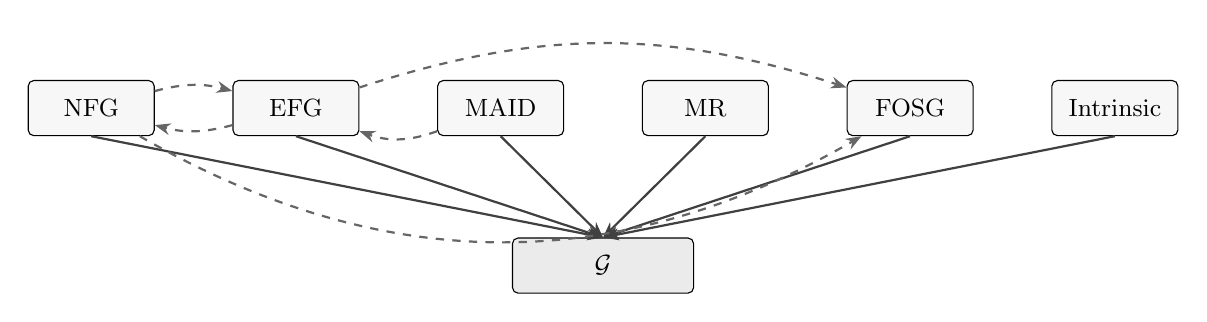
\begin{tikzpicture}[
  font=\small,
  box/.style = {draw, rounded corners=2pt, align=center,
                minimum height=0.7cm, minimum width=1.6cm,
                inner sep=3pt, fill=black!3},
  arr/.style = {-{Stealth[length=2mm]}, thick, black!75},
  brar/.style = {-{Stealth[length=2mm]}, thick, dashed, black!60},
]
\node[box] at (0, 1.4)   (nfg)  {NFG};
\node[box] at (2.6, 1.4) (efg)  {EFG};
\node[box] at (5.2, 1.4) (maid) {MAID};
\node[box] at (7.8, 1.4) (mr)   {MR};
\node[box] at (10.4,1.4) (fosg) {FOSG};
\node[box] at (13.0,1.4) (intr) {Intrinsic};

\node[box, fill=black!8, minimum width=2.3cm] at (6.5,-0.6) (kg) {\KG};

\foreach \src in {nfg, efg, maid, mr, fosg, intr} {
  \draw[arr] (\src.south) -- (kg.north);
}

\draw[brar, bend left=15] (nfg) to (efg);
\draw[brar, bend left=15] (efg) to (nfg);
\draw[brar, bend left=20] (maid) to (efg);
\draw[brar, bend left=18] (efg) to (fosg);
\draw[brar, bend right=30] (nfg) to (fosg);
\end{tikzpicture}
\end{center}

\noindent
Solid arrows are compilations $\compileTo$; dashed arrows are
bridges (\S\ref{sec:supp:bridges}).  The \emph{Repeated} and
\emph{Stochastic} languages are restrictions of MR and are not
shown separately.  Augmented EFG is a thin wrapper over EFG; it is
not a separate language.

\subsection{Code organization}
\label{sec:supp:code}

\begin{center}\small
\begin{tabular}{@{}p{0.22\textwidth}p{0.69\textwidth}@{}}
\toprule
Folder & Contents \\
\midrule
\TT{Math/} &
  Discrete-probability infrastructure that mathlib does not already
  provide:\ \DefRef{expect},
  \TT{Math.PMFProduct.pmfPi}, finsupp/finset update lemmas,
  optimization primitives. \\
\TT{Core/} &
  \DefRef{GameForm}, \DefRef{KernelGame}, the \DefRef{ProtocolMap}
  morphism vocabulary, simulations, isomorphisms, utility-invariance
  results. \\
\TT{Concepts/} &
  Solution concepts:\ Nash, dominance, best response, correlated /
  coarse correlated, Pareto, security, regret, approximate Nash,
  potential, zero-sum, team, symmetric, rationalizability, common
  knowledge, EU/preference properties. \\
\TT{Theorems/} &
  Major theorems:\ \DefRef{mixed_nash_exists},
  \DefRef{correlatedEq_exists}, \DefRef{von_neumann_minimax},
  \DefRef{zermelo}, \DefRef{oneShotDeviation_iff_spe}, the
  \DefRef{ObsModelCore} Kuhn theorems. \\
\TT{Languages/} &
  Six syntactic languages (NFG, EFG, MAID, MultiRound, FOSG,
  Intrinsic), each with its own \TT{Syntax}, \TT{Compile}, and
  worked-example files; bridges in \TT{Languages/Bridges/}. \\
\TT{Mechanism/} &
  Bayesian games, mechanism design, the revelation principle,
  social-choice fragments. \\
\TT{Auctions/} &
  Vickrey, FirstPrice, AllPay, VCG. \\
\bottomrule
\end{tabular}
\end{center}

% =====================================================================
\section{Probability infrastructure}
\label{sec:supp:probability}

The library uses mathlib's discrete probability monad
\TT{PMF} as its only distribution type.  This section documents
the few non-mathlib additions in \TT{Math/} that the rest of the
library depends on.

\subsection{Expected value: \TT{Math.Probability.expect}}
\label{sec:supp:expect}\label{def:expect}

\begin{leanbox}
namespace Math.Probability\\[1pt]
noncomputable def expect \{$\Omega$ : Type*\} (d : PMF $\Omega$) (f : $\Omega \to \mathbb{R}$) : $\mathbb{R}$ :=\\
\bd $\sum'\ \omega,\ (d\ \omega).\mathrm{toReal} * f\ \omega$\\[2pt]
theorem expect\_eq\_sum \{$\Omega$ : Type*\} [Fintype $\Omega$] (d : PMF $\Omega$) (f : $\Omega \to \mathbb{R}$) :\\
\bd expect d f = $\sum\ \omega : \Omega,\ (d\ \omega).\mathrm{toReal} * f\ \omega$\\[2pt]
@[simp] theorem expect\_pure \{$\Omega$ : Type*\} (f : $\Omega \to \mathbb{R}$) ($\omega$ : $\Omega$) :\\
\bd expect (PMF.pure $\omega$) f = f $\omega$
\end{leanbox}

\Mathematical
For a $\PMF{\Omega}$ given by mass function $d$ and a real-valued
function $f : \Omega \to \RR$,
\begin{equation}
\label{eq:supp:expect}
  \mathrm{expect}(d, f) \;=\; \sum_{\omega \in \Omega}^{\textsf{tsum}}
    d(\omega) \cdot f(\omega),
\end{equation}
where the sum is mathlib's \TT{tsum} (an unordered series with
non-negative-real summands; here the summands are real, but $d \ge 0$
and the unit-mass condition $\sum d = 1$ make absolute convergence
automatic for any bounded $f$, and the convention $\mathrm{tsum} = 0$
on non-summable inputs is harmless because we only call \TT{expect}
on bounded $f$).  When $\Omega$ is finite (the case used everywhere
in the library), \TT{expect_eq_sum} reduces this to an ordinary
finite sum.

\Textbook
This is the standard expected-value functional of the discrete
case (e.g.\ Maschler–Solan–Zamir~\citep{MaschlerSolanZamir2013}
§5.4 or Osborne–Rubinstein~\citep{OsborneRubinstein1994} §1.2).
The \TT{toReal} coercion is the only Lean-specific bookkeeping:\
\TT{PMF}'s mass function lands in $\overline{\RR}_{\ge 0}$
(extended non-negative reals) for technical mathlib reasons, and
\TT{toReal} brings it back to $\RR$.

\Faithfulness
Reformulation only.  The textbook expectation
$\mathbb{E}_\mu[f]$ is exactly \eqref{eq:supp:expect}; the
\TT{tsum} appears because mathlib's $\PMF$ is countably-supported
in general (the finite-support case is recovered automatically by
\TT{expect_eq_sum}).

\subsection{Finite product of PMFs: \texttt{Math.PMFProduct.pmfPi}}
\label{sec:supp:pmfpi}\label{def:pmfPi}

\begin{leanbox}
namespace Math.PMFProduct\\[1pt]
noncomputable def pmfPi \{$\iota$ : Type\} [Fintype $\iota$] \{$\alpha$ : $\iota \to$ Type\}\\
\bd ($\sigma$ : $\forall$ i, PMF ($\alpha$ i)) : PMF ($\forall$ i, $\alpha$ i)
\end{leanbox}

\Mathematical
For a finite family $\{\sigma_i \in \PMF{\alpha_i}\}_{i \in \Players}$,
$\mathrm{pmfPi}(\sigma)$ is the independent product distribution
on $\prod_i \alpha_i$,
\[
  \mathrm{pmfPi}(\sigma)(x) \;=\; \prod_{i \in \Players} \sigma_i(x_i).
\]
This is the canonical mixed-strategy joint distribution from
independent per-player mixings.

\Textbook
Standard:\ Osborne–Rubinstein §3.1 use it implicitly when defining
mixed-strategy equilibrium expected utility; we make it
explicit because the mixed extension of a kernel game
(\S\ref{sec:supp:mixedExtension}) needs it as a named operator.

\subsection{Other Math/ contents}
\label{sec:supp:math-other}

\TT{Math/Probability.lean} additionally contains the
\TT{Kernel}-as-function abbreviation $\mathrm{Kernel}\,A\,B = A \to
\PMF{B}$, the \TT{Kernel.pushforward} operator
(post-composition with a function, used to define
\TT{correlatedOutcome}), \TT{expect_bind} (linearity of
\TT{expect} along $\bind$), and \TT{expect_const} (expectation of
a constant function).  \TT{Math/PMFProduct.lean} adds the
projection laws of \TT{pmfPi}, in particular that
$\mathrm{pmfPi}(\sigma) \bind \pi_i = \sigma_i$ where $\pi_i$ is the
$i$-th coordinate projection.  These are routine and we do not
unfold them.

% =====================================================================
\section{The semantic core}
\label{sec:supp:core}

This section anchors the four objects on which the rest of the
library is built:\ \DefRef{GameForm}, \DefRef{KernelGame}, the
expected-utility functional \DefRef{KernelGame.eu}, and the
\DefRef{mixedExtension} construction.

\subsection{Game form: \texttt{GameForm}}
\label{sec:supp:gameform}\label{def:GameForm}

\Anchor{GameForm}
\begin{leanbox}
structure GameForm ($\iota$ : Type) where\\
\bd Strategy : $\iota \to$ Type\\
\bd Outcome  : Type\\
\bd outcomeKernel : Kernel ($\forall$ i, Strategy i) Outcome\\[3pt]
abbrev Profile (F : GameForm $\iota$) := $\forall$ i, F.Strategy i\\[3pt]
noncomputable def outcomeDist (F : GameForm $\iota$) ($\sigma$ : F.Profile) : PMF F.Outcome :=\\
\bd F.outcomeKernel $\sigma$\\[3pt]
noncomputable def correlatedOutcome (F : GameForm $\iota$) ($\mu$ : PMF F.Profile) : PMF F.Outcome :=\\
\bd Kernel.pushforward F.outcomeKernel $\mu$
\end{leanbox}

\Mathematical
A \emph{game form}~\citep{Myerson1991} over a player type
$\Players$ is the data
\[
  \GF \;=\; \bigl(\Strat : \Players \to \mathsf{Type},\;
                  \Outcome : \mathsf{Type},\;
                  \K : {\textstyle\prod_i}\Strat_i \to \PMF{\Outcome}\bigr).
\]
A \emph{strategy profile} is an element of $\prod_i \Strat_i$; a
\emph{correlated profile distribution} is an element of
$\PMF{\prod_i \Strat_i}$.  The kernel $\K$ assigns to each profile a
distribution over outcomes; the correlated outcome distribution is
the pushforward of the profile distribution along $\K$.

\Textbook
The protocol-only fragment of a game (Myerson §3.1; Maschler–
Solan–Zamir §1.2 call it the \emph{game form} explicitly).
Decomposing a game into protocol-only data and a separately
attached utility is standard mechanism-design practice; the Lean
record makes the decomposition structural (\TT{utility} is a field
of \DefRef{KernelGame}, not of \DefRef{GameForm}).

\Faithfulness
Reformulation.  The textbook game form is usually presented as the
strategy spaces and a deterministic outcome function or a
distributional version embedded in a larger structure; we expose
the distributional version directly because chance moves and
mixed strategies both produce $\PMF{\Outcome}$, and the cost of an
indirection through a deterministic outcome function plus an
external lift is exactly the indirection we wish to avoid
(see chapter \S3).

\Variants
\TT{Core/GameForm.lean} also defines:
\TT{deviateProfile} (unilateral coordinate update via
\TT{Function.update}); \TT{deviateOutcome},
\TT{deviateDistribution}, \TT{deviateDistributionFn} (push profile
or distribution through a deviation, by constant strategy or by a
function of the recommendation); \TT{constDeviateDistribution} and
its $\mathrm{Fn}$ variant; the bridge \TT{withUtility} adjoining a
utility (and the round-trip lemmas with \TT{toGameForm}); the
functorial action \TT{map} (post-composing a function on outcomes);
the \emph{independent product} of two game forms;
the \DefRef{ProtocolMap} morphism record (\S\ref{sec:supp:morphisms}).

\subsection{Kernel game: \texttt{KernelGame}}
\label{sec:supp:kernelgame}\label{def:KernelGame}

\Anchor{KernelGame}
\begin{leanbox}
abbrev Payoff ($\iota$ : Type) : Type := $\iota \to \mathbb{R}$\\[3pt]
structure KernelGame ($\iota$ : Type) where\\
\bd Strategy : $\iota \to$ Type\\
\bd Outcome  : Type\\
\bd utility  : Outcome $\to$ Payoff $\iota$\\
\bd outcomeKernel : Kernel ($\forall$ i, Strategy i) Outcome\\[3pt]
abbrev Profile (G : KernelGame $\iota$) := $\forall$ i, G.Strategy i\\[3pt]
def toGameForm (G : KernelGame $\iota$) : GameForm $\iota$ where\\
\bd Strategy := G.Strategy\\
\bd Outcome  := G.Outcome\\
\bd outcomeKernel := G.outcomeKernel
\end{leanbox}

\Mathematical
A \emph{kernel game} is a game form together with a utility
$\util : \Outcome \to \Players \to \RR$:
\[
  \KG \;=\; \bigl(\Strat,\;\Outcome,\;\util,\;\K\bigr),
  \qquad \util(\omega) \in \RR^\Players \text{ for each } \omega.
\]
The forgetful map $\toGF$ takes a kernel game to its game form;
its right adjoint \TT{withUtility} adjoins a utility back, and the
two compose to the identity in both directions.

\Textbook
This is the strategic-form game with stochastic outcome
mechanism — the most general finite strategic-form object:\ a
strategic-form game in the sense of
Osborne–Rubinstein~\citep{OsborneRubinstein1994} Definition 11.1
or Maschler–Solan–Zamir Definition 4.1, with the textbook
"deterministic action profile" replaced by a stochastic kernel.
A textbook normal-form game with utilities $u_i : A \to \RR$ is the
special case in which the kernel is the Dirac evaluation
$\Profile \mapsto \Dirac_\Profile$ (and the outcome type is $A$);
this is what the NFG language compiler produces.

\Faithfulness
Strict generalization in two directions.
\emph{(1)~Stochastic outcomes.}\ The textbook strategic form is
deterministic given a profile; we allow $\K(\Profile) \in
\PMF{\Outcome}$ to be any discrete distribution.  This subsumes
the deterministic case ($\K = \Dirac \circ f$ for a deterministic
$f$) and accommodates languages with chance moves (EFG, MAID,
MultiRound, FOSG) without an external lift.
\emph{(2)~Outcome type.}\ The textbook outcome is implicit (the
profile itself, or a payoff vector); we expose it as a parameter
\Outcome\ so that an EFG outcome (a terminal node in the tree) and
a NFG outcome (a joint action) can both inhabit \KG\ without
encoding tricks.

\Textbook (continued)
For a worked confirmation that \TT{IsNash} on a normal-form
game's compiled \KG\ unfolds to the textbook payoff inequality,
see \S\ref{sec:supp:examples:pd} (Prisoner's Dilemma).

\subsection{Expected utility: \texttt{KernelGame.eu}}
\label{sec:supp:eu}\label{def:KernelGame.eu}

\Anchor{KernelGame.eu}
\begin{leanbox}
noncomputable def eu (G : KernelGame $\iota$) ($\sigma$ : Profile G) (who : $\iota$) : $\mathbb{R}$ :=\\
\bd expect (G.outcomeKernel $\sigma$) (fun $\omega$ $\Rightarrow$ G.utility $\omega$ who)\\[3pt]
noncomputable def correlatedEu (G : KernelGame $\iota$)\\
\bd ($\mu$ : PMF (Profile G)) (who : $\iota$) : $\mathbb{R}$ :=\\
\bd expect (G.correlatedOutcome $\mu$) (fun $\omega$ $\Rightarrow$ G.utility $\omega$ who)
\end{leanbox}

\Mathematical
The expected utility of player $i$ under profile $\Profile$ in
kernel game $\KG$ is
\begin{equation}
\label{eq:supp:eu}
  \EU(\KG, \Profile, i) \;=\;
    \sum_{\omega \in \Outcome} \K(\Profile)(\omega) \cdot \util(\omega)(i),
\end{equation}
finite when \Outcome\ is finite.  In the general core API, this is
the tsum-based expectation over the discrete support.  The theorem
statements used in this chapter impose the finite hypotheses under
which this is the displayed finite sum.  The correlated variant is
the same expectation under the pushforward $\K_*\mu$ of a profile
distribution $\mu$.

\Textbook
The expected utility of a strategy profile in a strategic-form
game with stochastic outcome (vNM~\citep{vNM1944}, Theorem 1;
Maschler–Solan–Zamir §5.2).  The von Neumann–Morgenstern
expected-utility theorem is what \emph{justifies} taking
$\EU$ as the criterion of preference; the library's
$\IsNashFor$ predicate (\S\ref{sec:supp:isNash}) makes this
preference choice an explicit parameter so the EU criterion can
be replaced by another preorder if desired.

\Faithfulness
Reformulation.  The function \TT{expect}
(\S\ref{sec:supp:expect}) is exactly $\sum d(\omega)\,f(\omega)$
on a finite outcome space.  No measurability obligation arises
because \PMF\ is the discrete monad.

\subsection{Mixed extension: \texttt{KernelGame.mixedExtension}}
\label{sec:supp:mixedExtension}\label{def:mixedExtension}

\Anchor{KernelGame.mixedExtension}
\begin{leanbox}
open Classical in\\
noncomputable def mixedExtension (G : KernelGame $\iota$)\\
\bd [Fintype $\iota$] [$\forall$ i, Fintype (G.Strategy i)] : KernelGame $\iota$ where\\
\bd Strategy := fun i $\Rightarrow$ PMF (G.Strategy i)\\
\bd Outcome  := G.Outcome\\
\bd utility  := G.utility\\
\bd outcomeKernel := fun $\sigma$ $\Rightarrow$ (Math.PMFProduct.pmfPi $\sigma$).bind G.outcomeKernel
\end{leanbox}

\Mathematical
The mixed extension $\KG^{\mathrm{mix}}$ of a finite kernel game
$\KG$ has strategies $\PMF{\Strat_i}$ for each player, the same
outcome and utility, and the outcome kernel
\[
  \K^{\mathrm{mix}}(\Profile)
    \;=\; \mathrm{pmfPi}(\Profile) \mathbin{\bind} \K
    \;=\; \sum_{x \in \prod_i \Strat_i} \Bigl(\prod_i \Profile_i(x_i)\Bigr) \K(x).
\]
Independence of the per-player mixing is encoded in
\TT{pmfPi}; the original kernel $\K$ is then applied to the joint
pure profile drawn from this product.

\Textbook
The mixed extension of a finite game (Nash~\citep{Nash1951};
Osborne–Rubinstein Definition 32.1; Myerson §3.2):\ each player
randomizes independently over their pure strategies, and payoffs
are the expectation under the resulting product distribution.

\Faithfulness
Faithful.  The displayed formula is exactly the textbook one for
finite normal-form games; the only generalization is that
$\K$ may itself be stochastic (chance moves), in which case the
mixed extension's outcome kernel is the composition of the mixing
distribution with $\K$.  The classical case ($\K = \Dirac$) recovers
the textbook formula verbatim.

\subsection{Reindexing and \texttt{ofEU}: bunched}
\label{sec:supp:reindex-ofEU}

\begin{leanbox}
noncomputable def reindex \{$\iota\,\kappa$ : Type\} (e : $\iota \simeq \kappa$)\\
\bd (G : KernelGame $\kappa$) : KernelGame $\iota$\\[3pt]
noncomputable def KernelGame.ofEU\\
\bd (Strategy : $\iota \to$ Type)\\
\bd (eu : ($\forall$ i, Strategy i) $\to$ Payoff $\iota$) : KernelGame $\iota$
\end{leanbox}

\DefRef{reindex}\label{def:reindex} transports a kernel game across
a bijection of player types; this is presentation bookkeeping used
by bridges (\S\ref{sec:supp:bridges}) that canonicalize $\Players$
to $\mathrm{Fin}\,n$.  \DefRef{ofEU}\label{def:ofEU} constructs a
kernel game directly from a per-profile, per-player real-valued
function $\mathrm{eu} : \prod_i \Strat_i \to \Players \to \RR$ by
taking the outcome type to be $\Players \to \RR$ itself, the kernel
to be $\Profile \mapsto \Dirac_{\mathrm{eu}(\Profile)}$, and the
utility to be the identity.  The \TT{ofEU}-form is the natural
target of the Bayesian-game compilation
(\S\ref{sec:supp:bayesian}); structural lemmas in
\TT{Concepts/OfEUProperties.lean} record that
$\TT{eu}\,(\TT{ofEU}\,\TT{S}\,\TT{u})\,\sigma\,i = \TT{u}\,\sigma\,i$
and that solution-concept predicates on \TT{ofEU}-games unfold to
direct EU comparisons.

\subsection{Morphisms, simulations, isomorphisms}
\label{sec:supp:morphisms}\label{def:ProtocolMap}

\begin{leanbox}
structure ProtocolMap (F F' : GameForm $\iota$) where\\
\bd stratMap   : $\forall$ i, F.Strategy i $\to$ F'.Strategy i\\
\bd outcomeMap : F.Outcome $\to$ F'.Outcome\\
\bd outcomeKernel\_preserved : $\forall$ $\sigma$ : F.Profile,\\
\bdd F'.outcomeKernel (fun i $\Rightarrow$ stratMap i ($\sigma$ i)) =\\
\bdd \bd (F.outcomeKernel $\sigma$).bind (fun $\omega$ $\Rightarrow$ PMF.pure (outcomeMap $\omega$))\\[3pt]
def ProtocolMap.id  (F : GameForm $\iota$) : ProtocolMap F F\\
def ProtocolMap.comp (g : ProtocolMap F' F'') (f : ProtocolMap F F') : ProtocolMap F F''
\end{leanbox}

\Mathematical
A \emph{protocol map} from $\GF$ to $\GF'$ is a triple
$(\stratMap, \outcomeMap, \mathrm{preserved})$ satisfying the
\emph{outcome-kernel preservation} law:\ pushing a profile of $\GF$
through $\stratMap$ and then evaluating $\K'$ produces the same
distribution as evaluating $\K$ first and pushing the outcome
through $\outcomeMap$.  Equivalently, $\stratMap$ and $\outcomeMap$
form a coalgebra-style commuting square in the discrete Giry
monad.  Identity and composition exist and satisfy the standard
laws (\TT{ProtocolMap.id_comp}, \TT{comp_id}, \TT{comp_assoc}).

\Variants
\TT{KernelGame.Morphism} (\TT{Core/GameMorphism.lean}) is a protocol
map together with utility-preservation
$\util'(\outcomeMap(\omega))(i) = \util(\omega)(i)$.  A
\TT{KernelGame.Simulation} is a kernel-game morphism (the names
coincide).  A \TT{KernelGame.Bisimulation} is a simulation whose
strategy and outcome maps are bijective with simulation inverse;
it expresses an EU-isomorphism.  A
\TT{GameForm.ProtocolIsomorphism} is the analogous bijective
protocol-only version.  All of these come with \TT{id} and
\TT{comp} together with the corresponding identity/associativity
lemmas.

\Faithfulness
The morphism vocabulary is project-internal:\ no textbook canonizes
"protocol map between strategic-form games."  The categorical laws
are proved as \TT{simp}-lemmas (\TT{Core/GameForm.lean:307–349},
\TT{Core/GameMorphism.lean:67–77}); their content is the
distributional analogue of a coalgebra homomorphism.

% =====================================================================
\section{Solution concepts}
\label{sec:supp:solution-concepts}

This section catalogues the solution-concept predicates.  The
deviation-family schema of \S\ref{sec:supp:deviation-schema} is
the organizing principle:\ every equilibrium notion is an instance
of \TT{IsDeviationEqFamilyFor} for an explicit choice of
$\mathcal{D}$.  We anchor at $\IsNash$ (\S\ref{sec:supp:isNash})
and $\IsCorrelatedEq$ (\S\ref{sec:supp:isCE}); other concepts are
bunched.

\subsection{Deviation-family schema: \texttt{Core/GameForm.lean}}
\label{sec:supp:deviation-schema}\label{def:NoProfitableDeviationFor}\label{def:ProfileDeviationFamily}\label{def:IsDeviationEqFamilyFor}

\begin{leanbox}
namespace GameForm\\[1pt]
def NoProfitableDeviationFor (F : GameForm $\iota$)\\
\bd (pref : $\iota \to$ PMF F.Outcome $\to$ PMF F.Outcome $\to$ Prop)\\
\bd (who : $\iota$) (statusQuo : PMF F.Outcome)\\
\bd \{D : Type\} (deviate : D $\to$ PMF F.Outcome) : Prop :=\\
\bdd $\forall$ d : D, pref who statusQuo (deviate d)\\[3pt]
structure ProfileDeviationFamily (F : GameForm $\iota$) where\\
\bd Dev      : $\iota \to$ Type\\
\bd deviate  : PMF F.Profile $\to$ ($\forall$ who : $\iota$, Dev who $\to$ PMF F.Profile)\\[3pt]
def IsDeviationEqFamilyFor (F : GameForm $\iota$)\\
\bd (pref : $\iota \to$ PMF F.Outcome $\to$ PMF F.Outcome $\to$ Prop)\\
\bd ($\mu$ : PMF F.Profile) ($\Delta$ : ProfileDeviationFamily F) : Prop :=\\
\bdd $\forall$ who : $\iota$, F.NoProfitableProfileDeviationFor pref who $\mu$ ($\Delta$.deviate $\mu$ who)\\[3pt]
noncomputable def constantDeviationProfileFamily (F : GameForm $\iota$) : ProfileDeviationFamily F\\
noncomputable def recommendationDeviationFamily   (F : GameForm $\iota$) : ProfileDeviationFamily F
\end{leanbox}

\Mathematical
A \emph{deviation family} for player $i$ is a type $D_i$ of
deviations and a function transforming a profile distribution into
a deviated profile distribution given a deviation.  A profile
distribution $\mu$ is a $\mathcal{D}$-equilibrium for preference
$\Pref$ when no player has a profitable deviation in
$\mathcal{D}$:\
\[
  \forall i,\,\forall d \in D_i.\quad
    \Pref_i\bigl(\GF.\mathrm{correlatedOutcome}(\mu),\,
                 \GF.\mathrm{correlatedOutcome}(\mathrm{deviate}_i(\mu, d))\bigr).
\]
The two named families are
$\mathcal{D}^{\mathrm{const}}$ (deviations are constant
strategies; \TT{constantDeviationProfileFamily}) and
$\mathcal{D}^{\mathrm{dep}}$ (deviations are functions of the
recommendation; \TT{recommendationDeviationFamily}).

\Textbook
The deviation-family schema is project-internal but the two
families are textbook:\ unilateral deviation by a fixed strategy
(Nash, CCE) and recommendation-dependent deviation
(Aumann's correlated equilibrium~\citep{Aumann1974}).

\subsection{Deviation-simulation transport: \texttt{Concepts/DeviationSimulation.lean}}
\label{sec:supp:deviation-simulation}
\label{def:OutcomeView}\label{def:NashDeviationSimulation}\label{def:DeviationFamilySimulation}

\Anchor{OutcomeView}
\begin{leanbox}
structure OutcomeView (F : GameForm $\iota$) ($\Omega$ : Type) where\\
\bd observe : F.Outcome $\to$ $\Omega$\\[3pt]
def observedPref (V : OutcomeView F $\Omega$)\\
\bd (prefOmega : $\iota \to$ PMF $\Omega \to$ PMF $\Omega \to$ Prop) :\\
\bd $\iota \to$ PMF F.Outcome $\to$ PMF F.Outcome $\to$ Prop :=\\
\bdd fun who d e $\Rightarrow$ prefOmega who (PMF.map V.observe d) (PMF.map V.observe e)
\end{leanbox}

\Mathematical
An \emph{outcome view} records what part of a game's native outcome
is behaviorally relevant for a transport theorem.  If one
presentation returns terminal payoffs and another returns a richer
execution trace, both can be compared after projection to a common
carrier $\Omega$.  The induced preference
\TT{observedPref V prefOmega} compares native outcome laws only
through their pushforwards along \TT{V.observe}.  This is deliberately
more general than expected utility; the EU convenience
\TT{observedEuPref} is just the instance where \TT{prefOmega}
orders laws by expectation of a payoff function on $\Omega$.

\begin{leanbox}
structure ProfileRealization (G H : GameForm $\iota$) ($\Omega$ : Type) where\\
\bd viewG : OutcomeView G $\Omega$\\
\bd viewH : OutcomeView H $\Omega$\\
\bd rel   : G.Profile $\to$ H.Profile $\to$ Prop\\
\bd law\_eq : $\forall$ \{$\sigma$ : G.Profile\} \{$\tau$ : H.Profile\}, rel $\sigma$ $\tau$ $\to$\\
\bdd viewG.law $\sigma$ = viewH.law $\tau$\\[3pt]
structure NashDeviationSimulation (G H : GameForm $\iota$) ($\Omega$ : Type)\\
\bd extends ProfileRealization G H $\Omega$ where\\
\bd simulate\_target\_deviation :\\
\bdd $\forall$ \{$\sigma$ : G.Profile\} \{$\tau$ : H.Profile\}, rel $\sigma$ $\tau$ $\to$\\
\bdd $\forall$ (who : $\iota$) (sH : H.Strategy who),\\
\bdd $\exists$ sG : G.Strategy who,\\
\bdd viewG.law (Function.update $\sigma$ who sG) =\\
\bdd viewH.law (Function.update $\tau$ who sH)
\end{leanbox}

\Mathematical
\TT{ProfileRealization} is a relation, not a map, because many
semantic bridges are existential or many-to-many: a behavioral
profile may be realized by several mixed profiles, and a compiled
trace profile may forget administrative choices.  The base law
\TT{law_eq} says only that related profiles induce the same observed
status-quo law.  \TT{NashDeviationSimulation} adds the missing
equilibrium-relevant hypothesis: every unilateral deviation available
in the target presentation must be matched by some unilateral
deviation in the source presentation with the same observed law.

\begin{leanbox}
theorem NashDeviationSimulation.target\_nash\_of\_source\_nash\\
\bd (S : NashDeviationSimulation G H $\Omega$)\\
\bd (hrel : S.rel $\sigma$ $\tau$)\\
\bd (hN : G.IsNashFor (observedPref S.viewG prefOmega) $\sigma$) :\\
\bdd H.IsNashFor (observedPref S.viewH prefOmega) $\tau$
\end{leanbox}

\Mathematical
The proof is the two-line argument one expects.  Given a target
deviation $s_H$, use \TT{simulate_target_deviation} to obtain a
source deviation $s_G$.  The source Nash hypothesis compares the
source status quo with $s_G$; \TT{law_eq} rewrites the status quo to
the target law, and the simulation law rewrites the deviated law to
the target deviation.

\begin{leanbox}
structure ProfileDistributionRealization (G H : GameForm $\iota$) ($\Omega$ : Type) where\\
\bd viewG : OutcomeView G $\Omega$\\
\bd viewH : OutcomeView H $\Omega$\\
\bd rel   : PMF G.Profile $\to$ PMF H.Profile $\to$ Prop\\
\bd law\_eq : $\forall$ \{$\mu_G$ : PMF G.Profile\} \{$\mu_H$ : PMF H.Profile\}, rel $\mu_G$ $\mu_H$ $\to$\\
\bdd viewG.correlatedLaw $\mu_G$ = viewH.correlatedLaw $\mu_H$\\[3pt]
structure DeviationFamilySimulation\\
\bd (G H : GameForm $\iota$) ($\Omega$ : Type)\\
\bd ($\Delta_G$ : ProfileDeviationFamily G) ($\Delta_H$ : ProfileDeviationFamily H)\\
\bd extends ProfileDistributionRealization G H $\Omega$ where\\
\bd simulate\_target\_deviation :\\
\bdd $\forall$ \{$\mu_G$ : PMF G.Profile\} \{$\mu_H$ : PMF H.Profile\}, rel $\mu_G$ $\mu_H$ $\to$\\
\bdd $\forall$ (who : $\iota$) (dH : $\Delta_H$.Dev who),\\
\bdd $\exists$ dG : $\Delta_G$.Dev who,\\
\bdd viewG.correlatedLaw ($\Delta_G$.deviate $\mu_G$ who dG) =\\
\bdd viewH.correlatedLaw ($\Delta_H$.deviate $\mu_H$ who dH)
\end{leanbox}

\Mathematical
The family-level version moves from profiles to profile
distributions, because correlated and coarse correlated equilibrium
are predicates on a correlation device $\mu$.  The theorem
\TT{DeviationFamilySimulation.target_eq_of_source_eq} transports
\TT{IsDeviationEqFamilyFor}; the CE and CCE wrappers instantiate
$\Delta$ with \TT{recommendationDeviationFamily} and
\TT{constantDeviationProfileFamily}.  A two-way
\TT{DeviationFamilyBisimulation} packages simulations in both
directions and yields an iff.

\Faithfulness
No finiteness assumptions appear in these transport theorems.  They
use only exact equality of pushed-forward \TT{PMF} laws.  Finite
outcome hypotheses remain localized to existence theorems and to
expected-value lemmas that need finite sums.

% =====================================================================
\subsection{Nash equilibrium: \texttt{KernelGame.IsNash}}
\label{sec:supp:isNash}\label{def:KernelGame.IsNash}\label{def:IsNashFor}

\Anchor{KernelGame.IsNash}
\begin{leanbox}
open Classical in\\
def KernelGame.IsNash (G : KernelGame $\iota$) ($\sigma$ : Profile G) : Prop :=\\
\bd $\forall$ (who : $\iota$) (s' : G.Strategy who),\\
\bdd G.eu $\sigma$ who $\ge$ G.eu (Function.update $\sigma$ who s') who\\[3pt]
def KernelGame.IsNashFor (G : KernelGame $\iota$)\\
\bd (pref : $\iota \to$ PMF G.Outcome $\to$ PMF G.Outcome $\to$ Prop)\\
\bd ($\sigma$ : Profile G) : Prop :=\\
\bdd G.toGameForm.IsNashFor pref $\sigma$\\[3pt]
theorem KernelGame.IsNash\_iff\_IsNashFor\_eu (G : KernelGame $\iota$) ($\sigma$ : Profile G) :\\
\bd G.IsNash $\sigma$ $\leftrightarrow$ G.IsNashFor G.euPref $\sigma$
\end{leanbox}

\Mathematical
A profile $\Profile$ is a Nash equilibrium of $\KG$ when no player
has a strictly improving unilateral deviation:
\begin{equation}
\label{eq:supp:isNash}
  \forall i \in \Players,\,\forall s' \in \Strat_i.\quad
    \EU(\KG, \Profile, i) \;\ge\; \EU(\KG, \Profile[i \mapsto s'], i).
\end{equation}
The library's \TT{IsNashFor} variant
(\TT{Core/GameForm.lean}) generalizes \eqref{eq:supp:isNash} to
take an arbitrary preorder $\Pref$ on $\PMF{\Outcome}$:
\[
  \forall i,\,\forall s'.\quad \Pref_i\bigl(\K(\Profile),\;\K(\Profile[i \mapsto s'])\bigr).
\]
The bridge \TT{IsNash_iff_IsNashFor_eu} certifies that
$\IsNash$ is \TT{IsNashFor} instantiated at the EU preference
$\Pref^{\EU}$.

\Textbook
Osborne–Rubinstein Definition 14.1 (Nash equilibrium of a strategic
game):\ a strategy profile $a^*$ such that for every $i$ and every
$a_i \in A_i$, $u_i(a^*_{-i}, a_i^*) \ge u_i(a^*_{-i}, a_i)$.
Maschler–Solan–Zamir Definition 5.1 is identical with notation
$\sigma$ for the profile.  Myerson Definition 3.1 is the same
modulo the use of $\succsim$ in place of $\ge$ on real numbers.
\eqref{eq:supp:isNash} is verbatim these definitions specialized
to the EU preorder, with \TT{Function.update} encoding the
"$a^*_{-i}, a_i$" notation explicitly:\ \TT{Function.update $\sigma$ who s'}
is the profile that agrees with $\sigma$ at every coordinate except
\TT{who}, where it is replaced by \TT{s'}.

\Faithfulness
Faithful, with strict generalization through \TT{IsNashFor}.  The
weak-preference convention (the textbook uses $\ge$, the library
uses $\ge$ on EU; \TT{IsStrictNash} below uses $>$) matches the
weak Nash equilibrium of Osborne–Rubinstein 14.1.  See
\S\ref{sec:supp:examples:pd} for an end-to-end unfolding on
Prisoner's Dilemma:\ the predicate evaluates to four real
inequalities, one for each player and each alternative action,
exactly as in the textbook treatment.

\Variants
The bunched siblings of \TT{IsNash} are:
\begin{itemize}\itemsep1pt
\item \TT{IsBestResponse(For)} — a single coordinate is a best
  response against fixed opponents (the existential factor of
  Nash).
\item \TT{IsStrictNash(For)} — strict inequality for every $s' \neq
  \Profile_i$.
\item \TT{IsDominant(For)} / \TT{IsStrictDominant(For)} — the
  coordinate is best-response against \emph{every} opponent
  profile.
\item \TT{WeaklyDominates(For)} / \TT{StrictlyDominates(For)} —
  pairwise dominance as a binary predicate on strategies.
\end{itemize}
Each is the obvious quantifier rearrangement of \eqref{eq:supp:isNash}
and unfolds analogously.  The dominance$\Rightarrow$Nash chain
(\TT{KernelGame.dominant_is_nash}) and Nash$\Leftrightarrow$best-response
characterization are recorded as one-line corollaries.

% =====================================================================
\subsection{Correlated equilibrium: \texttt{KernelGame.IsCorrelatedEq}}
\label{sec:supp:isCE}\label{def:KernelGame.IsCorrelatedEq}

\Anchor{KernelGame.IsCorrelatedEq}
\begin{leanbox}
def IsCorrelatedEq (G : KernelGame $\iota$) ($\mu$ : PMF (Profile G)) : Prop := by\\
\bd classical\\
\bd exact $\forall$ (who : $\iota$) (dev : G.Strategy who $\to$ G.Strategy who),\\
\bdd G.correlatedEu $\mu$ who $\ge$\\
\bdd G.correlatedEu (G.unilateralDeviationDistribution $\mu$ who dev) who\\[3pt]
def IsCoarseCorrelatedEq (G : KernelGame $\iota$) ($\mu$ : PMF (Profile G)) : Prop := by\\
\bd classical\\
\bd exact $\forall$ (who : $\iota$) (s' : G.Strategy who),\\
\bdd G.correlatedEu $\mu$ who $\ge$\\
\bdd G.correlatedEu (G.constantDeviationDistribution $\mu$ who s') who
\end{leanbox}

\Mathematical
A profile distribution $\mu \in \PMF{\prod_i \Strat_i}$ is a
\emph{correlated equilibrium} of $\KG$ when, viewing $\mu$ as a
public correlation device privately recommending action $\mu_i$ to
each player, no player gains by replacing their recommendation by
any function of it:
\[
  \forall i,\,\forall \mathrm{dev} : \Strat_i \to \Strat_i.\quad
    \mathbb{E}_{\Profile \sim \mu}\bigl[u_i(\K(\Profile))\bigr]
    \;\ge\;
    \mathbb{E}_{\Profile \sim \mu}\bigl[u_i(\K(\Profile[i \mapsto \mathrm{dev}(\Profile_i)]))\bigr].
\]
\emph{Coarse correlated equilibrium}~\citep{HartMasColell2000}
restricts $\mathrm{dev}$ to constant functions $\mathrm{dev} \equiv s'$;
this corresponds to the deviation family
$\mathcal{D}^{\mathrm{const}}$ of
\S\ref{sec:supp:deviation-schema}.

\Textbook
Aumann~\citep{Aumann1974} Definition 2 (correlated equilibrium of
a finite Bayesian game with correlation device):\ for every
recommended action $a$, the conditional expectation under $\mu$ of
deviating to any $a' \neq a$ is no larger than the conditional
expectation of complying.  Our predicate is the (well-known)
equivalent ex-ante formulation:\ summing over all recommendations
of the conditional inequality gives \eqref{eq:supp:isNash}-style
total inequality on $\mu$, and the converse holds because the
conditional inequalities can be recovered by deviation functions
that act as the identity outside the conditioning event.

\Faithfulness
Faithful, with reformulation.  The library's
$\IsCorrelatedEq$ is the ex-ante form; the equivalent
ex-post (conditional) form is \TT{Concepts/CorrelatedEqProperties.lean}'s
\TT{isCorrelatedEq_iff_pointwise} (and similarly for the
preference-parameterized variant).  Existence is the content of
the main chapter's CE existence theorem
(\TT{KernelGame.correlatedEq_exists}).

\Variants
\TT{IsCorrelatedEqFor}, \TT{IsCoarseCorrelatedEqFor} are the
preference-parameterized versions; \TT{IsCorrelatedEqFor.toCoarseCorrelatedEqFor}
records the inclusion CE $\subseteq$ CCE; the schema instantiation
$\mu = \Dirac_\Profile$ recovers $\IsNashFor$ from
$\IsCoarseCorrelatedEqFor$.

% =====================================================================
\subsection{Other solution concepts: bunched}
\label{sec:supp:other-concepts}

We document the remaining concepts in groups.  Each group cites
its anchor textbook reference; the structural relation to
\IsNash\ or \IsCorrelatedEq\ is recorded in the prose.

\paragraph{Pareto and welfare.}\
\TT{Concepts/NashPareto.lean}, \TT{Concepts/WelfareTheorems.lean},
\TT{Concepts/PriceOfAnarchy.lean}.  \TT{ParetoDominatesFor} is the
binary preference-parameterized predicate "$\Profile$ Pareto-dominates
$\tau$"; \TT{IsParetoEfficient(For)} is its ¬∃-closure.
\TT{socialWelfare} is $\sum_i \EU(\KG, \Profile, i)$, requiring a
finite player set.  \TT{optimalWelfare}, \TT{worstNashWelfare},
\TT{bestNashWelfare} are the standard sup/inf over profile sets;
the Lean library does not yet package the ratio-valued
\TT{PoA}/\TT{PoS} definitions
(\citep{Koutsoupias1999, Roughgarden2005}).

\paragraph{Security and individual rationality.}\
\TT{Concepts/SecurityStrategy.lean}, \TT{Concepts/IndividualRationality.lean}.
\TT{securityLevel} of player $i$ is $\sup_s \inf_{\sigma_{-i}}
\EU(\KG, \sigma_{-i}[i \mapsto s], i)$; a security strategy
attains this supremum.  Individual rationality says no Nash payoff
is below the security level (Maschler–Solan–Zamir §5.4).

\paragraph{Regret.}\
\TT{Concepts/Regret.lean}.  External regret of $\Profile$ for $i$
is $\max_{s'}(\EU(\Profile[i\mapsto s'],i) - \EU(\Profile,i))^+$;
internal regret replaces $s'$ by a function of $\Profile_i$.  The
regret-equilibrium duality (zero average external regret iff CCE;
zero average internal regret iff CE) is recorded as
\TT{regret_zero_iff_isCoarseCorrelatedEq} and its CE analogue.

\paragraph{Approximate equilibria.}\
\TT{Concepts/ApproximateNash.lean}.  \TT{IsEpsilonNash $\varepsilon$}
relaxes the Nash inequality by an additive $\varepsilon$ slack;
$\varepsilon = 0$ recovers \TT{IsNash}.  Closure under
$\varepsilon$-relaxation extends to the deviation-family schema,
hence applies to $\varepsilon$-CCE and $\varepsilon$-CE.

\paragraph{Potential games.}\
\TT{Concepts/PotentialGame.lean}, \TT{PotentialFIP.lean},
\TT{PotentialWellFounded.lean}, \TT{PotentialTeam.lean}.
\TT{IsExactPotential $\Phi$} requires $\EU(\sigma',i) - \EU(\sigma,i) =
\Phi(\sigma') - \Phi(\sigma)$ for every unilateral deviation
$\sigma \to \sigma'$;  \TT{IsOrdinalPotential $\Phi$} replaces equality
by sign-equality.  \TT{IsExactPotential.toOrdinal} gives the
expected implication.  \TT{IsOrdinalPotential.nash_of_maximizer}:\
every $\Phi$-maximizer is Nash.  \TT{IsTeamGame.isExactPotential}:\
team games are exact potential games with $\Phi = u_{\mathrm{any}}$
(\citep{MonderShapley1996}).

\paragraph{Zero-sum, constant-sum, team, symmetric, evolutionary.}\
\TT{Concepts/ZeroSum.lean}, \TT{ConstantSum.lean},
\TT{TeamGame.lean}, \TT{SymmetricGame.lean},
\TT{EvolutionaryStability.lean}.  \TT{IsZeroSum}:\ $\sum_i \util(\omega)(i)
= 0$ for all $\omega$.  Constant-sum, team-game, and symmetric
predicates are similar.  \TT{ZeroSumNash}, \TT{ConstantSumNash}
record that two-player zero/constant-sum Nash profiles are exactly
the maximin/security profiles.  \TT{IsEvolutionarilyStable} is the
strict-dominance condition on a symmetric two-player game
(\citep{MaynardSmithPrice1973}).

\paragraph{Rationalizability and dominance solvability.}\
\TT{Concepts/Rationalizability.lean},
\TT{Concepts/DominanceSolvable.lean},
\TT{Concepts/DominanceSolvability.lean}.  \TT{Survives n} is the
predicate "survives $n$ rounds of iterated strict dominance
elimination," defined inductively;  \TT{IsRationalizable} is the
inf over $n$.  \TT{IsNash.isRationalizable} and
\TT{IsDominant.isRationalizable} are the expected implications.
\TT{Concepts/DominanceSolvable.lean} records that the unique
surviving profile (when one exists) is Nash.

\paragraph{Common knowledge.}\
\TT{Concepts/CommonKnowledge.lean}.  Aumann's common-knowledge
operator on a finite partition structure
(\citep{Aumann1976}); used as scaffolding for the mechanism layer.

% =====================================================================
\section{Languages}
\label{sec:supp:languages}

Each of the six languages in \TT{Languages/} ships with a
\TT{Syntax} file (the AST), often an \TT{SOS} operational
semantics, and a \TT{Compile} file producing a
\DefRef{KernelGame}.  This section anchors at the compilation
\emph{shape} for each language; full Syntax content beyond the
top-level record is bunched.

\subsection{NFG: \texttt{Languages/NFG/Compile.lean}}
\label{sec:supp:nfg}\label{def:NFG.NFGGame}\label{def:NFG.toKernelGame}

\Anchor{NFG.NFGGame.toKernelGame}
\begin{leanbox}
structure NFGGame ($\iota$ : Type) (A : $\iota \to$ Type) where\\
\bd Outcome  : Type\\
\bd outcome  : ($\forall$ i, A i) $\to$ Outcome\\
\bd utility  : ($\forall$ i, A i) $\to$ $\iota \to \mathbb{R}$\\[3pt]
noncomputable def NFGGame.toKernelGame (G : NFGGame $\iota$ A) : KernelGame $\iota$ where\\
\bd Strategy := A\\
\bd Outcome  := G.Outcome\\
\bd utility  := fun $\omega$ i $\Rightarrow$ \dots\\
\bd outcomeKernel := fun $\sigma$ $\Rightarrow$ PMF.pure (G.outcome $\sigma$)
\end{leanbox}

\Mathematical
A normal-form game over a finite player set $\Players$ and
action sets $\{A_i\}_i$ is the textbook tuple
$(\Players, \{A_i\}_i, \util)$.  The compiler takes the strategy
type to be $A_i$, the outcome type to be a chosen $\Outcome$ with
a deterministic projection from joint actions, and the kernel to
be the Dirac evaluation $\Profile \mapsto \Dirac_{G.\mathrm{outcome}(\Profile)}$.
The compiled \KG\ is deterministic; randomness enters only at the
mixed extension.  The structure does not impose finiteness on the
action types $A_i$ — countably infinite action spaces are
admitted at the definitional level (see
\TT{Languages/NFG/CountableExample.lean} for an $\mathbb{N}$-valued
smoke test); the mixed-Nash existence theorem reintroduces
\TT{[Fintype (A i)]} where the proof requires it.

\Textbook
Osborne–Rubinstein Definition 11.1 (strategic-form game).  The
compilation is the identity on the strategic form modulo the
choice of outcome type.

\Faithfulness
Faithful, with reformulation:\ the textbook treats utility as a
direct function of profile; we route through an outcome type so
that a kernel-game-level theorem applies uniformly to NFGs and to
languages with non-trivial outcome types.

\Variants
\TT{Languages/NFG/} also packages worked subclasses, each as its
own \TT{NFGGame} construction:\ \TT{CongestionGame.lean}
(Rosenthal's potential), \TT{CoalitionalGame.lean} (the Shapley
value definition plus null-player, additivity, linearity, and
symmetry lemmas),
\TT{Bargaining.lean} (Nash bargaining), \TT{Matching.lean}
(stable-matching predicates), \TT{PublicGoods.lean},
\TT{Stackelberg.lean}.  Each subclass lives in its own namespace
and exposes its characteristic theorem.

\subsection{EFG: \texttt{Languages/EFG/}}
\label{sec:supp:efg}\label{def:EFG.InfoStructure}\label{def:EFG.GameTree}\label{def:EFG.EFGGame}\label{def:EFG.evalDist}

\Anchor{EFG.GameTree, EFG.evalDist, EFG.toKernelGame}
\begin{leanbox}
structure InfoStructure where\\
\bd n        : Nat\\
\bd Infoset  : Fin n $\to$ Type\\
\bd arity    : (p : Fin n) $\to$ Infoset p $\to$ Nat\\
\bd arity\_pos : $\forall$ p I, 0 < arity p I\\[3pt]
inductive GameTree (S : InfoStructure) (Outcome : Type) where\\
\bd $\mid$ terminal (z : Outcome)\\
\bd $\mid$ chance (k : Nat) ($\mu$ : PMF (Fin k)) (hk : 0 < k) (next : Fin k $\to$ GameTree S Outcome)\\
\bd $\mid$ decision \{p : S.Player\} (I : S.Infoset p) (next : S.Act I $\to$ GameTree S Outcome)\\[3pt]
structure EFGGame where\\
\bd inf : InfoStructure ; Outcome : Type\\
\bd tree : GameTree inf Outcome ; utility : Outcome $\to$ Payoff inf.Player\\[3pt]
noncomputable def GameTree.evalDist \{S : InfoStructure\} \{Outcome : Type\}\\
\bd ($\sigma$ : BehavioralProfile S) : GameTree S Outcome $\to$ PMF Outcome\\
\bd $\mid$ .terminal z $\Rightarrow$ PMF.pure z\\
\bd $\mid$ .chance \_ $\mu$ \_ next $\Rightarrow$ $\mu$.bind (fun b $\Rightarrow$ (next b).evalDist $\sigma$)\\
\bd $\mid$ .decision (p := p) I next $\Rightarrow$ ($\sigma$ p I).bind (fun a $\Rightarrow$ (next a).evalDist $\sigma$)
\end{leanbox}

\Mathematical
An extensive-form game is a triple $(\InfoStruct, \Tree, \util)$
where \InfoStruct\ records the players, their information sets,
and the action arity at each information set; the tree is
inductively built from terminal, chance, and decision nodes; and
the utility maps terminal outcomes to payoff vectors.  Strategies
come in three flavors:\ pure
$\Spure_p = \forall I, \mathrm{Fin}(\mathrm{arity}(p, I))$,
behavioral $\Sbeh_p = \forall I, \PMF{\mathrm{Fin}(\mathrm{arity}(p, I))}$,
and mixed $\Smix_p = \PMF{\Spure_p}$.  The function \TT{evalDist}
evaluates the tree under a behavioral profile to a $\PMF{\Outcome}$
by structural recursion:\ chance binds the chance distribution,
decision binds the player's behavioral distribution at the
relevant information set, terminal returns Dirac.  The compiled
kernel game has \TT{Strategy} the behavioral type, the EFG outcome
as outcome, \TT{evalDist} as kernel, and the EFG utility as utility.

\Textbook
Kuhn's representation~\citep{Kuhn1953}; Osborne–Rubinstein Chapter
6.  The \TT{InfoStructure} factoring through information-set IDs
(rather than directly through a player type) is a presentation
choice for the type theory:\ a decision node stores only its
information-set ID, and the player is recovered from the
information structure.  Augmented EFGs in the FOSG-paper
sense~\citep{Kovarik2022} are a thin wrapper adding public and
per-player history partitions (\TT{Languages/EFG/Augmented.lean}).

\Faithfulness
Faithful, with reformulation:\ distributional semantics rather
than deterministic-with-lift.  See chapter §3.2 for the
rationale.  Subgame-perfect equilibrium
(\TT{EFG.EFGGame.IsSubgamePerfectEq} in
\TT{Languages/EFG/Refinements.lean}) is defined as a Nash
equilibrium of every subgame; the ODP characterization
(\S\ref{sec:supp:odp}) makes this a one-shot deviation check.

\Variants
\TT{Languages/EFG/} contains \TT{Augmented.lean} (the augmented
EFG), \TT{SOS.lean} (operational semantics for the tree),
\TT{Compile.lean} and \TT{CompileObs.lean} (the latter compiling
to ObsModelCore for Kuhn), \TT{Kuhn.lean} (language-level Kuhn
specialization), \TT{Refinements.lean} (subgame perfection,
behavioral/pure refinements), \TT{Examples.lean}, \TT{Tests.lean}.

\subsection{MAID: \texttt{Languages/MAID/}}
\label{sec:supp:maid}\label{def:MAID.MAIDGame}

\Anchor{MAID.MAIDGame.toKernelGame}
\begin{leanbox}
structure MAIDGame where\\
\bd Players      : Type ; [fin : Fintype Players]\\
\bd Node         : Type\\
\bd parents      : Node $\to$ Finset Node\\
\bd nodeKind     : Node $\to$ NodeKind  -- chance, decision, utility\\
\bd domain       : Node $\to$ Type ; chanceDist, decisionInfo, utilityFn fields\\
\bd acyclic      : ...\\[3pt]
noncomputable def MAIDGame.toKernelGame (G : MAIDGame) : KernelGame G.Players
\end{leanbox}

\Mathematical
A multi-agent influence diagram~\citep{KollerMilch2003} is a
directed acyclic graph whose nodes are typed as chance, decision,
or utility, with edges encoding informational and causal
dependence.  The compiler implements a \emph{frontier evaluator}
that, at each step, picks a node whose parents are all assigned and
either samples its chance distribution, consults the player's
strategy at the relevant decision node, or accumulates its
utility.  Order-independence (the diamond lemma in
\TT{MAID/FrontierLemmas.lean}) makes the compilation
well-defined.

\Textbook
Koller–Milch Definition 1; Pfeffer–Gal Section 2.  The Lean
formalization restricts to finite-domain MAIDs (each node has a
\TT{Fintype} domain).  Strategic-relevance and d-separation
analyses, prominent in the MAID literature, are not formalized;
the order-independence content is.

\Faithfulness
Faithful, with restriction to finite-domain nodes.  See chapter
§5.4 for the rationale on why we accepted the proof obligations of
order-independent compilation rather than fixing a topological
order.

\Variants
\TT{Languages/MAID/} contains \TT{Syntax.lean}, \TT{SOS.lean},
\TT{FrontierEval.lean}, \TT{FrontierLemmas.lean},
\TT{FoldEval.lean}, \TT{Prefix.lean} (subdiagram framework),
\TT{Compile.lean}, \TT{CompileObs.lean}, \TT{Kuhn.lean},
\TT{Theorems.lean}.

\subsection{MultiRound: \texttt{Languages/MultiRound/}}
\label{sec:supp:mr}\label{def:MultiRoundGame}

\Anchor{MultiRoundGame, Round}
\begin{leanbox}
structure Round (n : Nat) (S V A Sig : Type) where\\
\bd signal     : S $\to$ PMF (Fin n $\to$ Sig)\\
\bd view       : Fin n $\to$ S $\to$ Sig $\to$ V\\
\bd transition : S $\to$ (Fin n $\to$ Option A) $\to$ S\\[3pt]
structure MultiRoundGame (n : Nat) (S V A Sig : Type) where\\
\bd init   : S\\
\bd rounds : List (Round n S V A Sig)\\[3pt]
noncomputable def MultiRoundGame.toKernelGame
\end{leanbox}

\Mathematical
A multi-round game is an initial state and a finite list of rounds
\citep{ShohamLeytonBrown2008}.  Each round samples a joint signal
from a state-dependent distribution, lets each player observe their
own state-and-signal-derived view, and applies a deterministic
transition keyed on the joint optional action.  Strategies are pure
and memoryless at the protocol level — a function from view to
optional action — with mixed/behavioral and recall structure
imposed externally.  The compilation generates the outcome kernel
by folding the round list and threading the state through the
chain of observations and transitions.

\Variants
\TT{Languages/MultiRound/RepeatedGame.lean} restricts to identical
rounds; \TT{StochasticGame.lean}~\citep{Shapley1953stochastic}
specializes the transition to be itself stochastic and
state-conditioned.  \TT{CompileObs.lean} and its linearizations
(\TT{CompileObsLin.lean}, \TT{CompileObsLinAdequacy.lean},
\TT{CompileObsLinRecall.lean}) compile to the
\DefRef{ObsModelCore} substrate that the Kuhn theorem
(\S\ref{sec:supp:kuhn}) is stated against.

\subsection{FOSG: \texttt{Languages/FOSG/}}
\label{sec:supp:fosg}\label{def:FOSG}

\Anchor{FOSG.toKernelGame}
\begin{leanbox}
structure FOSG ($\iota$ W A : Type) (Obs : $\iota \to$ Type) (Pub : Type) where\\
\bd init             : W\\
\bd active           : W $\to$ Finset $\iota$\\
\bd availableActions : (w : W) $\to \iota \to$ Set A\\
\bd terminal         : W $\to$ Prop\\
\bd transition       : ...\\
\bd reward, privObs, pubObs : ...\\
\bd terminal\_active\_eq\_empty : ...\\
\bd terminal\_no\_legal, nonterminal\_exists\_legal : ...\\[3pt]
noncomputable def FOSG.toKernelGame (G : FOSG \dots) [BoundedHorizon] : KernelGame $\iota$
\end{leanbox}

\Mathematical
A factored-observation stochastic game~\citep{Kovarik2022} is the
most general of the language layers:\ a state space, an active-set
function (the players who must move at each state), per-player
available actions, a transition kernel, a reward vector, a per-
player private observation, and a public observation.  Strategies
are functions of observation sequences; histories are recorded by
an explicit \TT{History} type.  Bounded horizon makes the
compilation finite.

\Textbook
Kovařík et al.~\citep{Kovarik2022} Definition 1.

\Variants
\TT{Languages/FOSG/} contains \TT{Basic.lean}, \TT{History.lean},
\TT{Information.lean}, \TT{Strategy.lean}, \TT{Values.lean},
\TT{Execution.lean}, \TT{OutcomeClosure.lean}, \TT{Serial.lean},
\TT{Compile.lean}, \TT{Kuhn.lean}, \TT{Theorems.lean}, with the
canonical \DefRef{ObsModelCore} bridge in \TT{Theorems/Kuhn/}.

\subsection{Intrinsic-form: \texttt{Languages/Intrinsic/}}
\label{sec:supp:intrinsic}

\Anchor{Intrinsic.productMixedToBehavioral}
\begin{leanbox}
structure WGame where\\
\bd Players, Agents : Type\\
\bd agentPlayer : Agents $\to$ Players\\
\bd Action : Agents $\to$ Type ; ...\\
\bd InfoStructure : ...\\[3pt]
noncomputable def productMixedToBehavioral (G : WGame) : ...\\
theorem behavioral\_realizes\_productMixed (G : WGame) : ...
\end{leanbox}

\Mathematical
The intrinsic (Witsenhausen-style) representation of a game
\citep{HeymannDeLaraChancelier2020} exposes agent decision
\emph{addresses} and information sets directly, without fixing an
order in which agents act.  Three strategy types are defined:\
\emph{mixed} (a distribution over a player's joint pure strategy
space $\prod_{a \in A_p} \Lambda_a$), \emph{product-mixed}
(independent randomization over each address), and
\emph{behavioral} (independent randomization at each information
set).  The unconditional product-mixed/behavioral equivalence is
the intrinsic-form analogue of one direction of Kuhn's theorem and
holds without any recall hypothesis.

\Textbook
Heymann–De Lara–Chancelier 2020 Definitions 8, 10, 11; Propositions
12, 13.  The intrinsic layer is structurally a separate syntactic
root than the EFG/MAID/MR/FOSG family.

% =====================================================================
\section{Bridges}
\label{sec:supp:bridges}

Bridges between languages are commuting-compilation theorems; the
expressiveness lens of \TT{Languages/Expressiveness/} packages
them in a uniform shape.

\subsection{Languages and reductions: anchor}
\label{sec:supp:expressiveness}\label{def:Expressiveness.Language}\label{def:Expressiveness.Reduction}

\Anchor{Expressiveness.Language, Expressiveness.Reduction}
\begin{leanbox}
namespace GameTheory.Languages.Expressiveness\\[1pt]
structure Language ($\iota$ : Type) where\\
\bd Syntax  : Type u\\
\bd compile : Syntax $\to$ KernelGame $\iota$\\[3pt]
structure Reduction \{$\iota$ : Type\} (L : Language $\iota$) (M : Language $\iota$)\\
\bd (R : KernelGame $\iota$ $\to$ KernelGame $\iota$ $\to$ Prop) where\\
\bd translate : L.Syntax $\to$ M.Syntax\\
\bd sound     : $\forall$ x : L.Syntax, R (L.compile x) (M.compile (translate x))
\end{leanbox}

\Mathematical
A \emph{language} for a fixed player type $\Players$ is a syntax
class together with a compilation $\compileTo : \mathrm{Syntax} \to
\KG_\Players$.  A \emph{reduction} from $L$ to $M$ over a semantic
relation $R$ is a translation on syntax together with a proof that
the compiled games are $R$-related for every source program.
Reductions compose under transitivity of $R$.

\Variants
The relation taxonomy in \TT{Expressiveness/Relations.lean}
catalogues:
$\mathrm{ProtocolEquivalent}$ (game-form-level isomorphism,
ignoring utility); $\mathrm{UtilityDistributionEquivalent}$
(bisimulation; both protocol and joint utility distribution
preserved); $\mathrm{UtilityDistributionSimulation}$ (the directed
version); $\mathrm{EUEquivalent}$ (equal expected utility for each
player at corresponding profiles); $\mathrm{EUSimulation}$ (directed
EU-comparison; equilibria of the source pull back to the target).
The bridges of the next subsection are reductions in this lens.

\subsection{Concrete bridges: bunched}
\label{sec:supp:concrete-bridges}

\paragraph{NFG → EFG (\TT{Languages/Bridges/NFG_EFG.lean}).}\
Each finite NFG is presented as a depth-1 EFG with a single
information set per player and a flat tree of $|\Act_i|$ branches
at each.  Soundness at the EU-isomorphism level.

\paragraph{NFG → FOSG (\TT{Languages/Bridges/NFG_FOSG.lean}).}\
Each finite NFG is presented as a one-shot FOSG with two world
states ($\mathsf{init}, \mathsf{terminal}$), every player active
at $\mathsf{init}$, no observations, and a single deterministic
transition delivering the NFG payoff as the FOSG reward.
Soundness:\
\TT{NFGGame.toFOSG_terminal_iff} and the corresponding EU
equivalence.

\paragraph{EFG → NFG (\TT{Languages/Bridges/EFG_NFG.lean}).}\
The strategic form of a finite EFG:\ pure strategy = function from
information set to action, payoff = expected payoff under the
behavioral lift of that pure strategy.  Soundness at the
EU-equivalence level.

\paragraph{MAID → EFG (\TT{Languages/Bridges/MAID_EFG.lean}).}\
A bounded MAID compiles to an EFG via a topological scheduling of
its decision nodes; soundness at the strategic-form refinement
level (information sets preserved).

\paragraph{EFG → FOSG (\TT{Languages/Bridges/FOSG/}).}\
\TT{ObsModelCore.lean}, \TT{AugmentedEFG.lean},
\TT{SerialExec.lean}.  An EFG with serial execution is presented
as an FOSG.  Soundness at the game-form simulation level.

\subsection{Solution-concept transport}
\label{sec:supp:transport}

The main chapter's map-based transport theorem
(\TT{Core/UtilityInvariance.lean}) states that a protocol map with
bijective \TT{stratMap} and bijective \TT{outcomeMap} transports the
preference-parameterized Nash, best-response, dominance,
weak/strict dominance, correlated-equilibrium, and
coarse-correlated-equilibrium predicates pointwise across the
bijection on profiles.  Specializing to a kernel-game simulation
(utility-preserving) yields the EU-specific transport laws.

The observed-law transport layer
(\TT{Concepts/DeviationSimulation.lean}) removes the need for an
outcome bijection.  It compares two games through views into a
common observed carrier $\Omega$, relates profiles or profile
distributions by equality of the pushed-forward outcome law, and
requires one-way simulation of target deviations by source
deviations.  Under these hypotheses, Nash and arbitrary
\TT{ProfileDeviationFamily} equilibria transfer from source to
target; a two-way simulation gives an iff.  These results are the
operational content of bridges whose target presentation contains
extra trace data or serialized administrative structure:\ a Nash
equilibrium of the abstract source remains Nash after compilation
provided all compiled unilateral deviations are observed already by
some source-side unilateral deviation.

% =====================================================================
\section{Major theorems}
\label{sec:supp:theorems}

\subsection{Mixed Nash existence: \texttt{KernelGame.mixed\_nash\_exists\_of\_bounded}}
\label{sec:supp:nash-exists}\label{def:mixed_nash_exists}

\Anchor{mixed_nash_exists_of_bounded, mixed_nash_exists}
\begin{leanbox}
theorem KernelGame.mixed\_nash\_exists\_of\_bounded (G : KernelGame $\iota$)\\
\bd [Fintype $\iota$] [DecidableEq $\iota$]\\
\bd [$\forall$ i, Finite (G.Strategy i)] [$\forall$ i, Nonempty (G.Strategy i)]\\
\bd \{$C$ : $\iota \to \mathbb{R}$\} (hbd : $\forall$ who $\omega$, |G.utility $\omega$ who| $\le$ C who) :\\
\bd $\exists$ $\sigma$ : $\forall$ i, PMF (G.Strategy i),\ G.mixedExtension.IsNash $\sigma$\\[3pt]
theorem KernelGame.mixed\_nash\_exists (G : KernelGame $\iota$)\\
\bd [Fintype $\iota$] [DecidableEq $\iota$]\\
\bd [$\forall$ i, Finite (G.Strategy i)] [$\forall$ i, Nonempty (G.Strategy i)]\\
\bd [Finite G.Outcome] :\\
\bd $\exists$ $\sigma$ : $\forall$ i, PMF (G.Strategy i),\ G.mixedExtension.IsNash $\sigma$
\end{leanbox}

\Mathematical
Every finite-strategy game with bounded player utilities has a
mixed Nash equilibrium.  Hypotheses:\ finite player type,
decidable equality on players, finite non-empty strategy space per
player, and a playerwise bound $|\util(\omega,i)| \le C_i$.
The outcome carrier need not be finite.  The theorem
\TT{mixed_nash_exists} is the finite-outcome wrapper that derives
boundedness automatically.

\paragraph{Proof structure.}\
The proof follows Nash's gain-map argument~\citep{Nash1951}.
Define
$\mathrm{gain}_i(\Profile, s) = \EU(\KG^{\mathrm{mix}}, \Profile[i \mapsto \Dirac_s], i) - \EU(\KG^{\mathrm{mix}}, \Profile, i)$,
the gain to player $i$ from deviating to pure $s$, and
\[
  \Phi_i(\Profile)(s) \;=\;
    \frac{\Profile_i(s) + (\mathrm{gain}_i(\Profile, s))^+}
         {1 + \sum_{s'} (\mathrm{gain}_i(\Profile, s'))^+}.
\]
$\Phi$ is a continuous self-map of the product simplex
$\prod_i \Delta(\Strat_i)$.  Brouwer's fixed-point theorem (mathlib's
\TT{brouwerFixedPoint} on a closed disk, lifted to the product
simplex via the homeomorphism in
\TT{Concepts/ProductSimplexBrouwer.lean}) gives a fixed point
$\Profile^*$.  The algebraic step in
\TT{Theorems/NashExistenceMixed.lean} (section
\TT{NashMapAlgebra}) shows that a fixed point of $\Phi$ is a Nash
equilibrium:\ the positive-part bracketing forces every player's
gain to vanish at $\Profile^*$.

\Textbook
Nash 1951 Theorem 1; Osborne–Rubinstein Proposition 33.1.

\Faithfulness
Faithful.  The library is honest about non-constructivity:\
\TT{mixed_nash_exists_of_bounded} is \TT{noncomputable} because Brouwer is.
A constructive route via Sperner's lemma is listed in chapter
§10 as a future direction.

\subsection{Correlated and coarse correlated equilibrium existence}
\label{sec:supp:ce-exists}\label{def:correlatedEq_exists}

\begin{leanbox}
theorem KernelGame.correlatedEq\_exists\_of\_bounded       (G : KernelGame $\iota$) [...]
theorem KernelGame.correlatedEq\_exists                   (G : KernelGame $\iota$) [...]
theorem KernelGame.coarseCorrelatedEq\_exists\_of\_bounded (G : KernelGame $\iota$) [...]
theorem KernelGame.coarseCorrelatedEq\_exists             (G : KernelGame $\iota$) [...]
\end{leanbox}

The independent product
$\bigotimes_i \Profile^*_i$ over the mixed Nash profile supplied by
the main chapter's mixed-existence theorem is a correlated equilibrium
of the original \KG;\ this is the route taken by
\TT{Theorems/CorrelatedEqExistence.lean}.  CCE existence is the
corollary $\Pref$-CE $\subseteq$ $\Pref$-CCE.  See chapter §6.2
for the alternative no-regret-learning route, not formalized.  The
\TT{\_of\_bounded} statements require finite strategy spaces but
not finite outcomes.

\subsection{Minimax theorem: \texttt{KernelGame.von\_neumann\_minimax\_of\_bounded}}
\label{sec:supp:minimax}\label{def:von_neumann_minimax}

\Anchor{von_neumann_minimax_of_bounded, von_neumann_minimax}
\begin{leanbox}
theorem KernelGame.von\_neumann\_minimax\_of\_bounded (G : KernelGame (Fin 2))\\
\bd [$\forall$ i, Finite (G.Strategy i)] [$\forall$ i, Nonempty (G.Strategy i)]\\
\bd (hzs : G.IsZeroSum)\\
\bd \{$C$ : Fin 2 $\to \mathbb{R}$\} (hbd : $\forall$ i $\omega$, |G.utility $\omega$ i| $\le$ C i) :\\
\bd $\exists$ (v : $\mathbb{R}$) ($\sigma$ : Profile G.mixedExtension),\\
\bdd G.mixedExtension.IsNash $\sigma$ $\wedge$ G.mixedExtension.eu $\sigma$ 0 = v $\wedge$\\
\bdd ($\forall$ s$_1$, G.mixedExtension.eu (Function.update $\sigma$ 1 s$_1$) 0 $\ge$ v) $\wedge$\\
\bdd ($\forall$ s$_0$, G.mixedExtension.eu (Function.update $\sigma$ 0 s$_0$) 0 $\le$ v)\\[3pt]
theorem KernelGame.von\_neumann\_minimax (G : KernelGame (Fin 2))\\
\bd [Finite G.Outcome] [$\forall$ i, Finite (G.Strategy i)] [$\forall$ i, Nonempty (G.Strategy i)]\\
\bd (hzs : G.IsZeroSum) :\\
\bd $\exists$ (v : $\mathbb{R}$) ($\sigma$ : Profile G.mixedExtension),\\
\bdd G.mixedExtension.IsNash $\sigma$ $\wedge$ G.mixedExtension.eu $\sigma$ 0 = v $\wedge$\\
\bdd ($\forall$ s$_1$, G.mixedExtension.eu (Function.update $\sigma$ 1 s$_1$) 0 $\ge$ v) $\wedge$\\
\bdd ($\forall$ s$_0$, G.mixedExtension.eu (Function.update $\sigma$ 0 s$_0$) 0 $\le$ v)
\end{leanbox}

\Mathematical
Every finite-strategy two-player zero-sum game with bounded utility
has a mixed Nash profile whose player-0 payoff is a saddle value:\
player 1 cannot lower it by deviating and player 0 cannot raise it
by deviating.  A separate lemma records that all mixed Nash equilibria yield the same
expected utility for player 0.  The usual finite-game
max-min/min-max equality is the textbook reading of these saddle
inequalities, but it is not the literal statement packaged here.

\paragraph{Proof structure.}\
Existence of a mixed Nash profile is \TT{mixed_nash_exists_of_bounded}.
Equality of EU at any two Nash profiles is the saddle-point
property of zero-sum Nash, recorded as
\TT{IsZeroSum.nash_eu_eq_of_bounded} in \TT{Theorems/Minimax.lean}.

\Textbook
von Neumann 1928~\citep{vN1928}; Maschler–Solan–Zamir Theorem 7.6.

\subsection{Backward induction (Zermelo) and the ODP}
\label{sec:supp:odp}\label{def:zermelo}\label{def:oneShotDeviation_iff_spe}\label{def:HasNoOneShotDeviation}

\Anchor{HasNoOneShotDeviation, oneShotDeviation_iff_spe, zermelo}
\begin{leanbox}
def HasNoOneShotDeviation (G : EFGGame)\\
\bd ($\sigma$ : PureProfile G.inf) : Prop :=\\
\bd $\forall$ \{p\} (I : G.inf.Infoset p) (next : G.inf.Act I $\to$ GameTree G.inf G.Outcome),\\
\bdd ($\exists$ h, ReachBy h G.tree (.decision I next)) $\to$\\
\bdd $\forall$ a' : G.inf.Act I,\\
\bdd \bd expect ((next ($\sigma$ p I)).evalDist (pureToBehavioral $\sigma$)) (G.utility · p) $\ge$\\
\bdd \bd expect ((next a').evalDist (pureToBehavioral $\sigma$)) (G.utility · p)\\[3pt]
theorem oneShotDeviation\_iff\_spe\_of\_bounded (G : EFGGame)\\
\bd ($\sigma$ : PureProfile G.inf) (hpi : IsPerfectInfo G.tree)\\
\bd \{$C$ : G.inf.Player $\to \mathbb{R}$\} (hbd : $\forall$ p $\omega$, |G.utility $\omega$ p| $\le$ C p) :\\
\bd G.IsSubgamePerfectEq $\sigma$ $\leftrightarrow$ HasNoOneShotDeviation G $\sigma$\\[3pt]
theorem zermelo\_of\_bounded (G : EFGGame) (hpi : IsPerfectInfo G.tree)\\
\bd \{$C$ : G.inf.Player $\to \mathbb{R}$\} (hbd : $\forall$ p $\omega$, |G.utility $\omega$ p| $\le$ C p) :\\
\bd $\exists$ $\sigma$ : PureProfile G.inf, G.IsSubgamePerfectEq $\sigma$
\end{leanbox}

\Mathematical
The one-shot deviation principle:\ in a finite perfect-information
EFG, a pure profile is subgame-perfect iff it has no profitable
one-shot deviation at any reachable decision node.  Zermelo's
theorem:\ every finite perfect-information EFG has a pure
subgame-perfect equilibrium, constructed by backward induction.
The displayed theorems are the bounded-utility forms; finite
outcome wrappers \TT{oneShotDeviation\_iff\_spe} and \TT{zermelo}
derive boundedness automatically.

\paragraph{Proof structure.}\
\TT{Theorems/Zermelo.lean}.
\TT{perfectInfo_disjoint_subtrees}:\ in a perfect-info tree,
sibling subtrees have disjoint information-set supports, so
backward induction can fix actions at one decision node without
affecting optimality elsewhere.  \TT{exists_noOSD}:\ the inductive
backward construction yields a profile with no profitable one-shot
deviation.  Zermelo follows from \TT{exists_noOSD} and the ODP.

\Textbook
Zermelo 1913 (the chess theorem); modern treatment in
Selten 1965~\citep{Selten1965, Selten1975}; Osborne–Rubinstein
Chapter 6.4.  ODP is folklore (see Fudenberg–Tirole §3.3 for a
modern statement).

\subsection{Kuhn's theorem: \texttt{Theorems/Kuhn/}}
\label{sec:supp:kuhn}\label{def:ObsModelCore}\label{def:kuhn_behavioral_to_mixed}\label{def:kuhn_mixed_to_behavioral_semantic}

\Anchor{ObsModelCore, kuhn_behavioral_to_mixed, kuhn_mixed_to_behavioral_semantic}
\begin{leanbox}
structure ObsModelCore ($\iota\,\sigma$ : Type) (Obs : $\iota \to$ Type)\\
\bd (Act : (i : $\iota$) $\to$ Obs i $\to$ Type) where\\
\bd  -- world state, transition kernel, per-player observation, ...\\[3pt]
def NoNontrivialInfoStateRepeat (O : ObsModelCore ...) : Prop\\
def HorizonSeparation                (O : ObsModelCore ...) : Prop\\
def ActionPosteriorLocal            (O : ObsModelCore ...) : Prop\\
def PerStepPlayerRecall             (O : ObsModelCore ...) : Prop\\[3pt]
theorem ObsModelCore.kuhn\_behavioral\_to\_mixed\\
\bd (O : ObsModelCore ...) [...] (hH : HorizonSeparation O) (hR : NoNontrivialInfoStateRepeat O) :\\
\bd $\forall$ $\beta$ : BehavioralProfile O,\ runDist O $\beta$ = (behavioralToMixedJoint $\beta$).bind (runDistPure O)\\[3pt]
theorem ObsModelCore.kuhn\_mixed\_to\_behavioral\_semantic\\
\bd (O : ObsModelCore ...) [...] (hL : ActionPosteriorLocal O) :\\
\bd $\forall$ $\mu$ : PMF (PureProfile O), $\exists$ $\beta$, runDist O $\beta$ = $\mu$.bind (runDistPure O)
\end{leanbox}

\Mathematical
The library proves Kuhn's behavioral$\,\leftrightarrow\,$mixed
equivalence at a representation-neutral substrate, the
\TT{ObsModelCore} record:\ a tuple recording the world state, each
player's observation type, the per-observation action arity, and
a transition kernel.  Behavioral profiles are per-player
$\InfoState_i \to \PMF{\Act_i}$; mixed profiles are per-player
distributions over the deterministic functions
$\InfoState_i \to \Act_i$.

The four hypothesis predicates control which direction of Kuhn
applies:
\begin{itemize}\itemsep1pt
\item \emph{NoNontrivialInfoStateRepeat}:\ no information state
  is visited twice along any trace (except at trivially-arity
  states).  This enforces tree-shaped reachability and is needed
  for the $B \to M$ direction's product-of-information-states
  construction to be well-defined.
\item \emph{HorizonSeparation}:\ a sequential separation of
  histories by depth, also needed for $B \to M$.
\item \emph{ActionPosteriorLocal}:\ the conditional distribution
  of an action given an information state does not depend on
  information outside the player's recall.  Sufficient for $M \to
  B$.  Strictly weaker than perfect recall in the textbook sense.
\item \emph{PerStepPlayerRecall}:\ the syntactic version of
  ActionPosteriorLocal that is automatic for snapshot-refined
  information states.
\end{itemize}

The $B \to M$ direction (\TT{kuhn_behavioral_to_mixed}) constructs
the equivalent mixed profile by the independent product of the
behavioral distributions across information states; the
$M \to B$ direction (\TT{kuhn_mixed_to_behavioral_semantic})
constructs the behavioral profile by extracting the
information-state-conditional distributions from $\mu$.

\Textbook
Kuhn 1953 Theorem 4 (perfect-recall version); Aumann 1964 (recall
hypothesis sharpening); Selten 1975 §6 (textbook treatment).

\Faithfulness
Strict generalization.  The textbook Kuhn's theorem requires
perfect recall; the library proves both directions under
strictly weaker hypotheses.  The $B \to M$ direction needs no
recall at all; the $M \to B$ direction needs only
ActionPosteriorLocal, which holds whenever the information
structure has the per-step locality property — a condition
strictly weaker than full perfect recall.  See chapter §6.5 for
the rationale.

\Variants
\TT{Theorems/Kuhn/} contains the proof split:\
\TT{ObsModel.lean} (the snapshot-refined wrapper),
\TT{KuhnModel.lean} (alternative carrier),
\TT{BehavioralToMixedCore.lean}
(the $B \to M$ proof, ~613 lines),
\TT{MixedToBehavioralCore.lean} (the $M \to B$ proof, ~951 lines),
\TT{CorrelatedRealization.lean} (an alternative
$M \to B$ proof via the correlated-equilibrium realization formula).
The package also exposes generic outcome-equality schemas
(\TT{KuhnBehavioralToMixedOutcome},
\TT{KuhnMixedToBehavioralViaOutcome},
\TT{KuhnCompleteViaOutcome} in \TT{Theorems/Kuhn.lean}) for
language-specific Kuhn instantiations.

% =====================================================================
\section{Mechanism design and auctions}
\label{sec:supp:mechanism}

\subsection{Bayesian games: \texttt{Mechanism/BayesianGame.lean}}
\label{sec:supp:bayesian}\label{def:BayesianGame}\label{def:BayesianGame.toKernelGame}

\Anchor{BayesianGame, BayesianGame.toKernelGame}
\begin{leanbox}
structure BayesianGame ($\iota$ : Type) [Fintype $\iota$] where\\
\bd $\Theta$       : $\iota \to$ Type ; [Fintype, Nonempty]\\
\bd Act     : $\iota \to$ Type ; [Fintype, Nonempty]\\
\bd prior   : PMF ($\forall$ i, $\Theta$ i)\\
\bd utility : ($\forall$ i, $\Theta$ i) $\to$ ($\forall$ i, Act i) $\to \iota \to \mathbb{R}$\\[3pt]
abbrev Strategy (B : BayesianGame $\iota$) (i : $\iota$) := B.$\Theta$ i $\to$ B.Act i\\[3pt]
noncomputable def exAnteEU (B : BayesianGame $\iota$) ($\sigma$ : B.BProfile) (who : $\iota$) : $\mathbb{R}$ :=\\
\bd expect B.prior (fun $\theta$ $\Rightarrow$ B.utility $\theta$ (fun i $\Rightarrow$ $\sigma$ i ($\theta$ i)) who)\\[3pt]
noncomputable def toKernelGame (B : BayesianGame $\iota$) : KernelGame $\iota$ :=\\
\bd KernelGame.ofEU B.Strategy (fun $\sigma$ i $\Rightarrow$ B.exAnteEU $\sigma$ i)\\[3pt]
def BayesNash (B : BayesianGame $\iota$) ($\sigma$ : B.BProfile) : Prop :=\\
\bd B.toKernelGame.IsNash $\sigma$\\[3pt]
theorem bayesNash\_iff\_exAnteEU (B : BayesianGame $\iota$) ($\sigma$ : B.BProfile) :\\
\bd B.BayesNash $\sigma$ $\leftrightarrow$ $\forall$ (who) (s'), B.exAnteEU $\sigma$ who $\ge$ B.exAnteEU (Function.update $\sigma$ who s') who
\end{leanbox}

\Mathematical
A Bayesian game is a tuple
$(\Theta, \mathrm{Act}, \mu, u)$ with $\Theta_i$ the type space of
player $i$, $\mathrm{Act}_i$ the action space, $\mu \in
\PMF{\prod_i \Theta_i}$ the common prior, and $u$ the
type-and-action-dependent payoff.  A strategy is a function
$\Theta_i \to \mathrm{Act}_i$.  The compilation goes through
\TT{KernelGame.ofEU}:\ the strategy type is preserved, the outcome
type is $\Players \to \RR$, and the kernel is the Dirac evaluation
at the ex-ante expected utility \TT{exAnteEU}.  Bayes-Nash
equilibrium is exactly Nash on the compiled kernel game,
characterized concretely by \TT{bayesNash_iff_exAnteEU}.

\Textbook
Harsanyi 1967~\citep{Harsanyi1967} type-agent representation;
Osborne–Rubinstein Chapter 24.

\Faithfulness
Reformulation.  The textbook Bayesian Nash equilibrium quantifies
over type-conditional deviations; we use the equivalent ex-ante
formulation, where a deviation is a function $\Theta_i \to
\mathrm{Act}_i$ replacing the player's strategy globally.  The
ex-post and interim variants are derived definitions.
\emph{Restriction:}\ finite type and action spaces.

\subsection{General mechanisms and the revelation principle}
\label{sec:supp:revelation}\label{def:GeneralMechanism}\label{def:revelation_principle}

\Anchor{GeneralMechanism, revelation_principle}
\begin{leanbox}
structure GeneralMechanism ($\iota$ : Type) [Fintype $\iota$] where\\
\bd $\Theta$       : $\iota \to$ Type ; Act : $\iota \to$ Type\\
\bd outcome : ($\forall$ i, Act i) $\to \iota \to \mathbb{R}$\\[3pt]
def StrategyProfile (M : GeneralMechanism $\iota$) := $\forall$ i, M.$\Theta$ i $\to$ M.Act i\\[3pt]
def IsBNE (M : GeneralMechanism $\iota$) ($\mu$ : PMF ($\forall$ i, M.$\Theta$ i)) ($\sigma$ : M.StrategyProfile) : Prop\\[3pt]
noncomputable def toDirect (M : GeneralMechanism $\iota$) ($\sigma$ : M.StrategyProfile) : Mechanism $\iota$\\[3pt]
theorem revelation\_principle (M : GeneralMechanism $\iota$) ($\mu$ : PMF ($\forall$ i, M.$\Theta$ i))\\
\bd ($\sigma$ : M.StrategyProfile) (h : M.IsBNE $\mu$ $\sigma$) :\\
\bd (M.toDirect $\sigma$).isBIC $\mu$
\end{leanbox}

\Mathematical
A general mechanism has separate type spaces and action spaces;
strategies map types to actions.  A direct mechanism has
$\mathrm{Act}_i = \Theta_i$.  Bayesian incentive compatibility (BIC)
of a direct mechanism is BNE under truthful reporting.  The
revelation principle says:\ for any general mechanism with a BNE
$\sigma$, the direct mechanism that composes reports with $\sigma$
is BIC in the library's constant-misreport sense.

\Textbook
Myerson 1981~\citep{Myerson1981}; Maschler–Solan–Zamir Chapter
17.

\Faithfulness
Faithful to the finite direct-mechanism construction, with one
restriction:\ \TT{Mechanism.isBIC} quantifies over constant
misreports $\theta'_i$, whereas the stronger Bayes-Nash predicate
over the induced Bayesian game quantifies over arbitrary
type-dependent reporting strategies.  The library includes
\TT{isBIC_of_truthful_bayesNash} to relate the two levels.

\subsection{Auctions: bunched}
\label{sec:supp:auctions}\label{def:vickrey_truthful_dominant}

\Anchor{vickrey_truthful_dominant}
\begin{leanbox}
noncomputable def vickreyPayoff (v : Fin n $\to \mathbb{R}$) (bids : Fin n $\to \mathbb{R}$) (who : Fin n) : $\mathbb{R}$ :=\\
\bd if bids who > maxOtherBid bids who then v who - maxOtherBid bids who else 0\\[3pt]
theorem vickrey\_truthful\_dominant (v : Fin n $\to \mathbb{R}$) (who : Fin n) :\\
\bd $\forall$ bids b', vickreyPayoff v (Function.update bids who (v who)) who $\ge$\\
\bdd vickreyPayoff v (Function.update bids who b') who
\end{leanbox}

\Mathematical
In a second-price (Vickrey) auction with valuations $v$, the
payoff is $v_i - \max_{j \neq i} b_j$ for the highest bidder
($b_i$) if their bid strictly exceeds the rest, and $0$ otherwise.
Truthful bidding $b_i = v_i$ is a weakly dominant strategy:\ for
any opponents' bids and any alternative bid $b'$, the payoff under
truthful bidding is at least as large.

\Textbook
Vickrey 1961~\citep{Vickrey1961}.

\Faithfulness
Faithful.  The proof is a case analysis on whether $b'$ is above
or below $\max_{j \neq i} b_j$, in each case verifying that the
payoff under truthful bidding matches or exceeds.

\Variants
\TT{Auctions/FirstPrice.lean}, \TT{Auctions/AllPay.lean},
\TT{Auctions/VCG.lean}.  First-price constructs the deterministic
first-price payoff game and proves that no single bid is dominant.
All-pay records payoff facts such as overbidding being unprofitable
and rent dissipation.  VCG packages the efficient-allocation setup
and proves truthful reporting is dominant
(Clarke 1971, Groves 1973).

\subsection{Social choice}
\label{sec:supp:social-choice}

\TT{Mechanism/SocialChoice.lean} formalizes a finite set of
alternatives, a finite set of voters with strict preferences over
alternatives, and structural notions:\ preference profiles,
utilitarian aggregation, the existence of a welfare-maximizing
alternative.  The classical impossibility theorems (Arrow,
Gibbard–Satterthwaite, Sen) are not formalized; see chapter §10.

% =====================================================================
\section{Worked examples}
\label{sec:supp:examples}

The chapter's §6 (Worked example) traces Prisoner's Dilemma at a
high level.  This section gives the full Lean text and the
unfolding of the relevant predicates.

\subsection{Prisoner's Dilemma}
\label{sec:supp:examples:pd}

\begin{leanbox}
namespace NFG\\[1pt]
inductive PDAction where $\mid$ cooperate $\mid$ defect\\
deriving DecidableEq, Repr\\[3pt]
def prisonersDilemma : NFGGame Bool (fun \_ $\Rightarrow$ PDAction) where\\
\bd Outcome := $\forall$ \_ : Bool, PDAction\\
\bd outcome := id\\
\bd utility s p :=\\
\bdd match s true, s false, p with\\
\bdd $\mid$ defect, defect, true $\Rightarrow$ 1\\
\bdd $\mid$ cooperate, defect, true $\Rightarrow$ 0\\
\bdd $\mid$ defect, cooperate, true $\Rightarrow$ 3\\
\bdd $\mid$ cooperate, cooperate, true $\Rightarrow$ 2\\
\bdd $\mid$ ...\\[3pt]
def pd\_defect\_defect : StrategyProfile (fun \_ : Bool $\Rightarrow$ PDAction) :=\\
\bd fun \_ $\Rightarrow$ PDAction.defect\\[3pt]
theorem pd\_defect\_is\_nash : IsNashPure prisonersDilemma pd\_defect\_defect := by\\
\bd intro i a' ; cases i $<;>$ cases a' $<;>$\\
\bdd simp [prisonersDilemma, pd\_defect\_defect, deviate, Function.update]
\end{leanbox}

\paragraph{Faithfulness check.}\
The predicate \TT{IsNashPure prisonersDilemma pd_defect_defect}
unfolds (after \TT{intro i a'}) to four cases, one per
$(i \in \{T, F\}, a' \in \{C, D\})$ pair:
\begin{itemize}\itemsep1pt
\item $i = T, a' = C$:\ payoff at $(D, D)$ for player $T$ is $1$,
  payoff at $(C, D)$ for player $T$ is $0$.  $1 \ge 0$. \checkmark
\item $i = T, a' = D$:\ same profile.  $1 \ge 1$. \checkmark
\item $i = F, a' = C$:\ payoff at $(D, D)$ for $F$ is $1$, payoff
  at $(D, C)$ for $F$ is $0$.  $1 \ge 0$. \checkmark
\item $i = F, a' = D$:\ same profile.  $1 \ge 1$. \checkmark
\end{itemize}
Each inequality is the textbook Nash check.  The Lean proof closes
all four with one \TT{simp}.

The companion theorem \TT{pd_coop_not_nash} :\
\TT{¬ IsNashPure prisonersDilemma pd_coop_coop}
exhibits a profitable deviation:\ player $T$ deviates from $C$ to
$D$ and gains payoff $3 - 2 = 1$.  The Lean proof extracts the
$T$, $D$ instance of $\IsNash$, simplifies, and closes with
\TT{linarith}.

\subsection{Matching Pennies}
\label{sec:supp:examples:mp}

\begin{leanbox}
inductive MPAction where $\mid$ heads $\mid$ tails\\[3pt]
def matchingPennies : NFGGame Bool (fun \_ $\Rightarrow$ MPAction) where\\
\bd Outcome := $\forall$ \_ : Bool, MPAction\\
\bd outcome := id\\
\bd utility := -- (H,H) = (1,-1), (H,T) = (-1,1), ...
\end{leanbox}

\paragraph{Faithfulness check.}\
There is no pure Nash equilibrium:\ at $(H, H)$ player $F$ deviates
to $T$ and gains $+2$; at $(H, T)$ player $T$ deviates to $T$ and
gains $+2$; the four pure profiles are similarly checked.  The
textbook mixed equilibrium is the symmetric uniform profile
$\Profile^*_T = \Profile^*_F = \tfrac12 \Dirac_H + \tfrac12 \Dirac_T$,
at which both players' EU is $0$.  The Lean example records
the no-pure-Nash result; it does not package the mixed-equilibrium
calculation as a theorem in \TT{Languages/NFG/Examples.lean}.

\subsection{A two-step centipede in EFG}
\label{sec:supp:examples:centipede}

A two-step centipede:\ player 0 chooses Take or Pass; if Pass,
player 1 chooses Take or Pass; payoffs $\mathrm{TT_0} = (1, 0)$,
$\mathrm{PT} = (0, 2)$, $\mathrm{PP} = (3, 1)$.  The textbook
backward-induction solution is $(T, T)$:\ at the second node,
player 1 strictly prefers $T$ ($2 > 1$), so they play $T$; at the
first node, player 0 anticipates this and prefers $T$ ($1 > 0$).
The library's packaged extensive-form example is the entry-deterrence
game in \TT{Languages/EFG/Refinements.lean}, where it proves:
\begin{itemize}\itemsep1pt
\item \TT{entrySPE_isSPE}:\ the backward-induction profile is SPE.
\item \TT{entryNash_isNash}:\ another profile is Nash.
\item \TT{entryNash_not_spe}:\ that Nash profile is not SPE.
\end{itemize}
The two-step centipede calculation is illustrative prose, not a
separate Lean theorem.

\subsection{A small Bayesian game}
\label{sec:supp:examples:bayesian}

A two-player coordination game with binary types:\ each player has
type $\theta_i \in \{0, 1\}$ drawn independently uniform; actions
are $a_i \in \{L, R\}$; payoffs are $u_i(\theta, a) = [\![ a_T = a_F ]\!]
\cdot [\![ a_T = \theta_T ]\!]$.  The Bayes-Nash equilibrium has
each player play $a_i = \theta_i$;\ the Lean proof unfolds
\TT{bayesNash_iff_exAnteEU} and verifies the four-deviation
inequality directly under the uniform prior.

% =====================================================================
\section{Reading order}
\label{sec:supp:reading}

Three suggested traversals.

\paragraph{(a)~"I want to use the library on a finite NFG."}\
\S\ref{sec:supp:probability} (probability primitives) →
\S\ref{sec:supp:gameform}, \S\ref{sec:supp:kernelgame},
\S\ref{sec:supp:eu} (semantic core) →
\S\ref{sec:supp:isNash} (Nash) →
\S\ref{sec:supp:nfg} (NFG) →
\S\ref{sec:supp:nash-exists} (existence).
\S\ref{sec:supp:examples:pd} is the canonical worked example.

\paragraph{(b)~"I want to add a new language."}\
\S\ref{sec:supp:core} (semantic core) →
\S\ref{sec:supp:nfg} or \S\ref{sec:supp:efg} as a template →
\S\ref{sec:supp:expressiveness} (Language/Reduction abstraction)
to register the language for bridges.  The
worked subclass files inside \TT{Languages/NFG/} (CongestionGame,
Bargaining, Stackelberg) are useful as additional templates.

\paragraph{(c)~"I want to follow the Kuhn theorem proof end-to-end."}\
\S\ref{sec:supp:probability} → \S\ref{sec:supp:gameform},
\S\ref{sec:supp:kernelgame} → \S\ref{sec:supp:efg} (EFG behavioral
profiles) → \S\ref{sec:supp:kuhn} (the four hypotheses, then the
two anchor theorems).  The proof split is in
\TT{BehavioralToMixedCore.lean} and \TT{MixedToBehavioralCore.lean}
in \TT{Theorems/Kuhn/}; the
\TT{CorrelatedRealization.lean} alternative goes via the
mixed-Nash-induced correlated distribution.

\bibliographystyle{plainnat}
\bibliography{references}

\end{document}

